\documentclass[twoside]{book}

% Packages required by doxygen
\usepackage{fixltx2e}
\usepackage{calc}
\usepackage{doxygen}
\usepackage[export]{adjustbox} % also loads graphicx
\usepackage{graphicx}
\usepackage[utf8]{inputenc}
\usepackage{makeidx}
\usepackage{multicol}
\usepackage{multirow}
\PassOptionsToPackage{warn}{textcomp}
\usepackage{textcomp}
\usepackage[nointegrals]{wasysym}
\usepackage[table]{xcolor}

% Font selection
\usepackage[T1]{fontenc}
\usepackage[scaled=.90]{helvet}
\usepackage{courier}
\usepackage{amssymb}
\usepackage{sectsty}
\renewcommand{\familydefault}{\sfdefault}
\allsectionsfont{%
  \fontseries{bc}\selectfont%
  \color{darkgray}%
}
\renewcommand{\DoxyLabelFont}{%
  \fontseries{bc}\selectfont%
  \color{darkgray}%
}
\newcommand{\+}{\discretionary{\mbox{\scriptsize$\hookleftarrow$}}{}{}}

% Page & text layout
\usepackage{geometry}
\geometry{%
  a4paper,%
  top=2.5cm,%
  bottom=2.5cm,%
  left=2.5cm,%
  right=2.5cm%
}
\tolerance=750
\hfuzz=15pt
\hbadness=750
\setlength{\emergencystretch}{15pt}
\setlength{\parindent}{0cm}
\setlength{\parskip}{3ex plus 2ex minus 2ex}
\makeatletter
\renewcommand{\paragraph}{%
  \@startsection{paragraph}{4}{0ex}{-1.0ex}{1.0ex}{%
    \normalfont\normalsize\bfseries\SS@parafont%
  }%
}
\renewcommand{\subparagraph}{%
  \@startsection{subparagraph}{5}{0ex}{-1.0ex}{1.0ex}{%
    \normalfont\normalsize\bfseries\SS@subparafont%
  }%
}
\makeatother

% Headers & footers
\usepackage{fancyhdr}
\pagestyle{fancyplain}
\fancyhead[LE]{\fancyplain{}{\bfseries\thepage}}
\fancyhead[CE]{\fancyplain{}{}}
\fancyhead[RE]{\fancyplain{}{\bfseries\leftmark}}
\fancyhead[LO]{\fancyplain{}{\bfseries\rightmark}}
\fancyhead[CO]{\fancyplain{}{}}
\fancyhead[RO]{\fancyplain{}{\bfseries\thepage}}
\fancyfoot[LE]{\fancyplain{}{}}
\fancyfoot[CE]{\fancyplain{}{}}
\fancyfoot[RE]{\fancyplain{}{\bfseries\scriptsize Generated by Doxygen }}
\fancyfoot[LO]{\fancyplain{}{\bfseries\scriptsize Generated by Doxygen }}
\fancyfoot[CO]{\fancyplain{}{}}
\fancyfoot[RO]{\fancyplain{}{}}
\renewcommand{\footrulewidth}{0.4pt}
\renewcommand{\chaptermark}[1]{%
  \markboth{#1}{}%
}
\renewcommand{\sectionmark}[1]{%
  \markright{\thesection\ #1}%
}

% Indices & bibliography
\usepackage{natbib}
\usepackage[titles]{tocloft}
\setcounter{tocdepth}{3}
\setcounter{secnumdepth}{5}
\makeindex

% Hyperlinks (required, but should be loaded last)
\usepackage{ifpdf}
\ifpdf
  \usepackage[pdftex,pagebackref=true]{hyperref}
\else
  \usepackage[ps2pdf,pagebackref=true]{hyperref}
\fi
\hypersetup{%
  colorlinks=true,%
  linkcolor=blue,%
  citecolor=blue,%
  unicode%
}

% Custom commands
\newcommand{\clearemptydoublepage}{%
  \newpage{\pagestyle{empty}\cleardoublepage}%
}

\usepackage{caption}
\captionsetup{labelsep=space,justification=centering,font={bf},singlelinecheck=off,skip=4pt,position=top}

%===== C O N T E N T S =====

\begin{document}

% Titlepage & ToC
\hypersetup{pageanchor=false,
             bookmarksnumbered=true,
             pdfencoding=unicode
            }
\pagenumbering{roman}
\begin{titlepage}
\vspace*{7cm}
\begin{center}%
{\Large Byggern }\\
\vspace*{1cm}
{\large Generated by Doxygen 1.8.11}\\
\end{center}
\end{titlepage}
\clearemptydoublepage
\tableofcontents
\clearemptydoublepage
\pagenumbering{arabic}
\hypersetup{pageanchor=true}

%--- Begin generated contents ---
\chapter{Byggern}
\label{md_README}
\hypertarget{md_README}{}
This is the Byggern project...

This team is made up of Johan Lofstad, Sondre Baugstø and Sondre Vincent Russvoll. 



Documentation is available at \href{https://srussvoll.github.io/byggern/}{\tt https\+://srussvoll.\+github.\+io/byggern/}. 



The \textquotesingle{}build\textquotesingle{} folder contains all build files like .hex and .elf. The \textquotesingle{}include\textquotesingle{} folder contains all header files. The \textquotesingle{}lib\textquotesingle{} folder contains folders with libraries containing both source and header files. The \textquotesingle{}src\textquotesingle{} folder contains the source files. 



Added C++ support. Note that the S\+TL isn\textquotesingle{}t implemented. More specifically, only the C standard library is available... The new and delete operators are not implemented either, so just don\textquotesingle{}t use dynamic allocation without malloc(). Also remember that I\+S\+Rs are implemented in C with no support for overloading... Because of this interrupt handlers must be friends of the originator class. 
\chapter{Namespace Index}
\section{Namespace List}
Here is a list of all documented namespaces with brief descriptions\-:\begin{DoxyCompactList}
\item\contentsline{section}{\hyperlink{namespace_menu}{Menu} \\*This is a namespace containing everything needed to implement a menu. This namespace contains data types for describing a menu, and a controller class to control it and display it on a \hyperlink{class_o_l_e_d}{O\-L\-E\-D} (library class). The menu allocates \hyperlink{namespace_menu}{Menu} and \hyperlink{struct_menu_1_1_item}{Item} objects on the heap. Thus you should declare these objects O\-N T\-H\-E S\-T\-A\-C\-K I\-N\-S\-I\-D\-E A L\-O\-C\-A\-L S\-C\-O\-P\-E so the menus and menu items aren't stored both on the heap and in the main (or where the menu is created) stack! }{\pageref{namespace_menu}}{}
\item\contentsline{section}{\hyperlink{namespace_utilities}{Utilities} \\*Contains useful utilities for both the main program and libraries }{\pageref{namespace_utilities}}{}
\end{DoxyCompactList}

\chapter{Hierarchical Index}
\section{Class Hierarchy}
This inheritance list is sorted roughly, but not completely, alphabetically\+:\begin{DoxyCompactList}
\item \contentsline{section}{Menu\+:\+:Controller}{\pageref{class_menu_1_1_controller}}{}
\item \contentsline{section}{Menu\+:\+:Item}{\pageref{struct_menu_1_1_item}}{}
\item \contentsline{section}{Menu\+:\+:Menu}{\pageref{struct_menu_1_1_menu}}{}
\item \contentsline{section}{Stream}{\pageref{class_stream}}{}
\begin{DoxyCompactList}
\item \contentsline{section}{A\+DC}{\pageref{class_a_d_c}}{}
\item \contentsline{section}{O\+L\+ED}{\pageref{class_o_l_e_d}}{}
\item \contentsline{section}{U\+A\+RT}{\pageref{class_u_a_r_t}}{}
\end{DoxyCompactList}
\end{DoxyCompactList}

\chapter{Class Index}
\section{Class List}
Here are the classes, structs, unions and interfaces with brief descriptions\-:\begin{DoxyCompactList}
\item\contentsline{section}{\hyperlink{class_stream}{Stream} }{\pageref{class_stream}}{}
\item\contentsline{section}{\hyperlink{class_test_stream}{Test\-Stream} }{\pageref{class_test_stream}}{}
\end{DoxyCompactList}

\chapter{File Index}
\section{File List}
Here is a list of all documented files with brief descriptions\-:\begin{DoxyCompactList}
\item\contentsline{section}{include/{\bfseries init.\-h} }{\pageref{init_8h}}{}
\item\contentsline{section}{lib/adc/{\bfseries adc.\-h} }{\pageref{adc_8h}}{}
\item\contentsline{section}{lib/can/{\bfseries can.\-h} }{\pageref{can_8h}}{}
\item\contentsline{section}{lib/mcp2515/{\bfseries mcp2515.\-h} }{\pageref{mcp2515_8h}}{}
\item\contentsline{section}{lib/mcp2515/{\bfseries mcp2515\-\_\-regisers.\-h} }{\pageref{mcp2515__regisers_8h}}{}
\item\contentsline{section}{lib/menu/{\bfseries menu.\-h} }{\pageref{menu_8h}}{}
\item\contentsline{section}{lib/oled/\hyperlink{oled_8h}{oled.\-h} }{\pageref{oled_8h}}{}
\item\contentsline{section}{lib/spi/\hyperlink{spi_8h}{spi.\-h} }{\pageref{spi_8h}}{}
\item\contentsline{section}{lib/stream/\hyperlink{stream_8h}{stream.\-h} }{\pageref{stream_8h}}{}
\item\contentsline{section}{lib/uart/\hyperlink{uart_8h}{uart.\-h} }{\pageref{uart_8h}}{}
\item\contentsline{section}{lib/utilities/{\bfseries fonts.\-h} }{\pageref{fonts_8h}}{}
\item\contentsline{section}{lib/utilities/{\bfseries memory.\-h} }{\pageref{memory_8h}}{}
\item\contentsline{section}{lib/utilities/{\bfseries new.\-h} }{\pageref{new_8h}}{}
\item\contentsline{section}{lib/utilities/{\bfseries printf.\-h} }{\pageref{printf_8h}}{}
\item\contentsline{section}{lib/utilities/{\bfseries utilities.\-h} }{\pageref{utilities_8h}}{}
\end{DoxyCompactList}

\chapter{Namespace Documentation}
\hypertarget{namespace_utilities}{\section{Utilities Namespace Reference}
\label{namespace_utilities}\index{Utilities@{Utilities}}
}


Contains useful utilities for both the main program and libraries.  


\subsection*{Functions}
\begin{DoxyCompactItemize}
\item 
void \hyperlink{namespace_utilities_a7175bc91000cbd130685885c6a24ea9a}{Enable\-Printf} (\hyperlink{class_stream}{Stream} \&stream)
\end{DoxyCompactItemize}


\subsection{Detailed Description}
Contains useful utilities for both the main program and libraries. 

\subsection{Function Documentation}
\hypertarget{namespace_utilities_a7175bc91000cbd130685885c6a24ea9a}{\index{Utilities@{Utilities}!Enable\-Printf@{Enable\-Printf}}
\index{Enable\-Printf@{Enable\-Printf}!Utilities@{Utilities}}
\subsubsection[{Enable\-Printf}]{\setlength{\rightskip}{0pt plus 5cm}void Utilities\-::\-Enable\-Printf (
\begin{DoxyParamCaption}
\item[{{\bf Stream} \&}]{stream}
\end{DoxyParamCaption}
)}}\label{namespace_utilities_a7175bc91000cbd130685885c6a24ea9a}
Connects stdout to the specified stream, enabling printf(). 
\begin{DoxyParams}{Parameters}
{\em stream} & The stream stdio (printf) should use. \\
\hline
\end{DoxyParams}

\chapter{Class Documentation}
\hypertarget{class_a_d_c}{}\section{A\+DC Class Reference}
\label{class_a_d_c}\index{A\+DC@{A\+DC}}
Inheritance diagram for A\+DC\+:\begin{figure}[H]
\begin{center}
\leavevmode
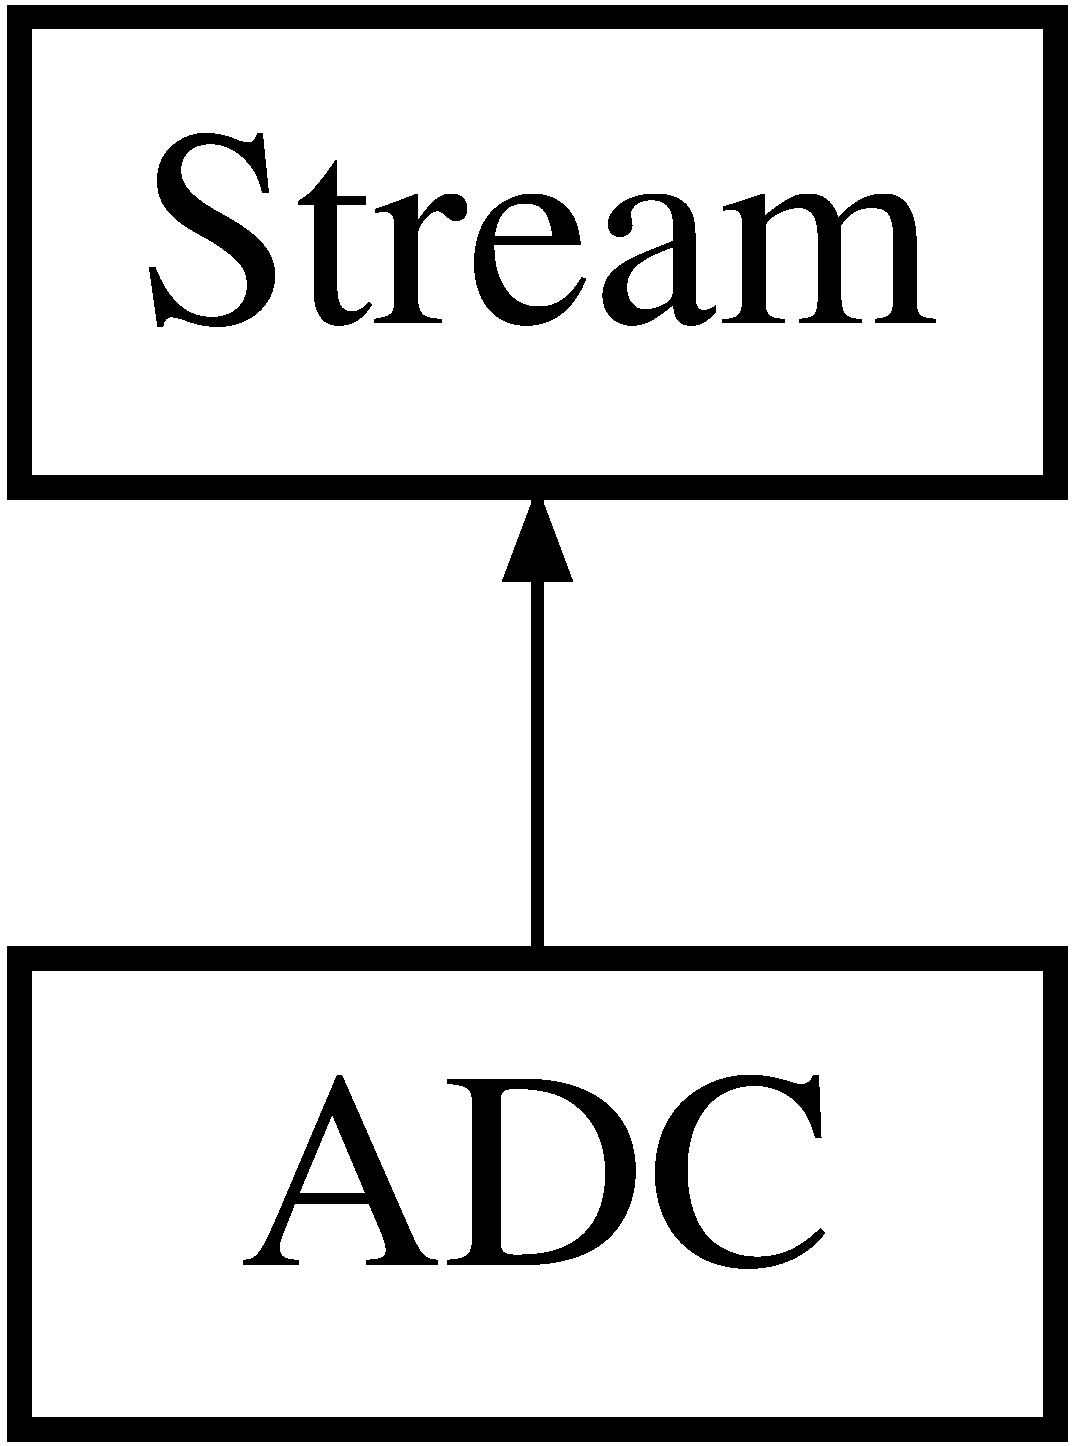
\includegraphics[height=2.000000cm]{class_a_d_c}
\end{center}
\end{figure}
\subsection*{Public Member Functions}
\begin{DoxyCompactItemize}
\item 
\hyperlink{class_a_d_c_a50cb1d4e5bb8e3812732d9efdde4af67}{A\+DC} (const \hyperlink{class_a_d_c}{A\+DC} \&)=delete
\item 
void \hyperlink{class_a_d_c_a8cc7efa85ad7492480bdfd9f49039150}{operator=} (const \hyperlink{class_a_d_c}{A\+DC} \&)=delete
\item 
bool \hyperlink{class_a_d_c_a8264cbf9141f229f5117718e78f01173}{request\+\_\+sample} ()
\end{DoxyCompactItemize}
\subsection*{Static Public Member Functions}
\begin{DoxyCompactItemize}
\item 
static \hyperlink{class_a_d_c}{A\+DC} \& \hyperlink{class_a_d_c_aa9294ebc0b114898aa33d9e09537bdb5}{Get\+Instance} (uint16\+\_\+t adc\+\_\+number, uint8\+\_\+t int\+\_\+pin)
\end{DoxyCompactItemize}
\subsection*{Static Public Attributes}
\begin{DoxyCompactItemize}
\item 
static bool \hyperlink{class_a_d_c_a861d0d9bd4dc73f9811c129548fb9a48}{adc\+\_\+in\+\_\+use} = false
\item 
\hypertarget{class_a_d_c_a472fee5492ee8e10d5baf38b67db18af}{}\label{class_a_d_c_a472fee5492ee8e10d5baf38b67db18af} 
static volatile uint8\+\_\+t $\ast$ {\bfseries adc\+\_\+waiting} = nullptr
\end{DoxyCompactItemize}
\subsection*{Private Member Functions}
\begin{DoxyCompactItemize}
\item 
\hyperlink{class_a_d_c_a0818050dee0dd8789966db0f429ef0bd}{A\+DC} (uint16\+\_\+t address, uint8\+\_\+t int\+\_\+pin)
\end{DoxyCompactItemize}
\subsection*{Private Attributes}
\begin{DoxyCompactItemize}
\item 
\hypertarget{class_a_d_c_aa58c27581281db4bd8537df9ea2b49f2}{}\label{class_a_d_c_aa58c27581281db4bd8537df9ea2b49f2} 
volatile uint8\+\_\+t $\ast$ {\bfseries address}
\end{DoxyCompactItemize}
\subsection*{Static Private Attributes}
\begin{DoxyCompactItemize}
\item 
\hypertarget{class_a_d_c_a6e0562436e7b39f0e53435ed5cc393a3}{}\label{class_a_d_c_a6e0562436e7b39f0e53435ed5cc393a3} 
static uint8\+\_\+t {\bfseries int\+\_\+pin} = 0
\end{DoxyCompactItemize}
\subsection*{Friends}
\begin{DoxyCompactItemize}
\item 
void \hyperlink{class_a_d_c_a8f7964aad4550f29972483135452c811}{I\+N\+T2\+\_\+vect} ()
\end{DoxyCompactItemize}
\subsection*{Additional Inherited Members}


\subsection{Constructor \& Destructor Documentation}
\hypertarget{class_a_d_c_a0818050dee0dd8789966db0f429ef0bd}{}\label{class_a_d_c_a0818050dee0dd8789966db0f429ef0bd} 
\index{A\+DC@{A\+DC}!A\+DC@{A\+DC}}
\index{A\+DC@{A\+DC}!A\+DC@{A\+DC}}
\subsubsection{\texorpdfstring{A\+D\+C()}{ADC()}\hspace{0.1cm}{\footnotesize\ttfamily [1/2]}}
{\footnotesize\ttfamily A\+D\+C\+::\+A\+DC (\begin{DoxyParamCaption}\item[{uint16\+\_\+t}]{address,  }\item[{uint8\+\_\+t}]{int\+\_\+pin }\end{DoxyParamCaption})\hspace{0.3cm}{\ttfamily [private]}}

Constructor for \hyperlink{class_a_d_c}{A\+DC} class. Singleton implementation 
\begin{DoxyParams}{Parameters}
{\em address} & The address the \hyperlink{class_a_d_c}{A\+DC} is located at. Channel on the adc is determined by the L\+SB. We use 0x1404 for channel 1 and 0x1405 for channel 2 \\
\hline
\end{DoxyParams}
\hypertarget{class_a_d_c_a50cb1d4e5bb8e3812732d9efdde4af67}{}\label{class_a_d_c_a50cb1d4e5bb8e3812732d9efdde4af67} 
\index{A\+DC@{A\+DC}!A\+DC@{A\+DC}}
\index{A\+DC@{A\+DC}!A\+DC@{A\+DC}}
\subsubsection{\texorpdfstring{A\+D\+C()}{ADC()}\hspace{0.1cm}{\footnotesize\ttfamily [2/2]}}
{\footnotesize\ttfamily A\+D\+C\+::\+A\+DC (\begin{DoxyParamCaption}\item[{const \hyperlink{class_a_d_c}{A\+DC} \&}]{ }\end{DoxyParamCaption})\hspace{0.3cm}{\ttfamily [delete]}}

Beacause of singleton -\/ makes sure its not copied etc. 

\subsection{Member Function Documentation}
\hypertarget{class_a_d_c_aa9294ebc0b114898aa33d9e09537bdb5}{}\label{class_a_d_c_aa9294ebc0b114898aa33d9e09537bdb5} 
\index{A\+DC@{A\+DC}!Get\+Instance@{Get\+Instance}}
\index{Get\+Instance@{Get\+Instance}!A\+DC@{A\+DC}}
\subsubsection{\texorpdfstring{Get\+Instance()}{GetInstance()}}
{\footnotesize\ttfamily static \hyperlink{class_a_d_c}{A\+DC}\& A\+D\+C\+::\+Get\+Instance (\begin{DoxyParamCaption}\item[{uint16\+\_\+t}]{adc\+\_\+number,  }\item[{uint8\+\_\+t}]{int\+\_\+pin }\end{DoxyParamCaption})\hspace{0.3cm}{\ttfamily [inline]}, {\ttfamily [static]}}

A Singleton implementation of this class. See \hyperlink{class_a_d_c}{A\+D\+C(uint16\+\_\+t address)} for more information. \hypertarget{class_a_d_c_a8cc7efa85ad7492480bdfd9f49039150}{}\label{class_a_d_c_a8cc7efa85ad7492480bdfd9f49039150} 
\index{A\+DC@{A\+DC}!operator=@{operator=}}
\index{operator=@{operator=}!A\+DC@{A\+DC}}
\subsubsection{\texorpdfstring{operator=()}{operator=()}}
{\footnotesize\ttfamily void A\+D\+C\+::operator= (\begin{DoxyParamCaption}\item[{const \hyperlink{class_a_d_c}{A\+DC} \&}]{ }\end{DoxyParamCaption})\hspace{0.3cm}{\ttfamily [delete]}}

Beacause of singleton -\/ makes sure its not copied etc. \hypertarget{class_a_d_c_a8264cbf9141f229f5117718e78f01173}{}\label{class_a_d_c_a8264cbf9141f229f5117718e78f01173} 
\index{A\+DC@{A\+DC}!request\+\_\+sample@{request\+\_\+sample}}
\index{request\+\_\+sample@{request\+\_\+sample}!A\+DC@{A\+DC}}
\subsubsection{\texorpdfstring{request\+\_\+sample()}{request\_sample()}}
{\footnotesize\ttfamily bool A\+D\+C\+::request\+\_\+sample (\begin{DoxyParamCaption}{ }\end{DoxyParamCaption})}

Request the \hyperlink{class_a_d_c}{A\+DC} to get a sample. This sample can be read from the buffer using \hyperlink{class_stream_a6db4180f5834073f992608b856bddca2}{Read\+Byte(uint8\+\_\+t\& byte)}; 

\subsection{Friends And Related Function Documentation}
\hypertarget{class_a_d_c_a8f7964aad4550f29972483135452c811}{}\label{class_a_d_c_a8f7964aad4550f29972483135452c811} 
\index{A\+DC@{A\+DC}!I\+N\+T2\+\_\+vect@{I\+N\+T2\+\_\+vect}}
\index{I\+N\+T2\+\_\+vect@{I\+N\+T2\+\_\+vect}!A\+DC@{A\+DC}}
\subsubsection{\texorpdfstring{I\+N\+T2\+\_\+vect}{INT2\_vect}}
{\footnotesize\ttfamily void I\+N\+T2\+\_\+vect (\begin{DoxyParamCaption}{ }\end{DoxyParamCaption})\hspace{0.3cm}{\ttfamily [friend]}}

The interrupt vector for \hyperlink{class_a_d_c}{A\+DC} done 

\subsection{Member Data Documentation}
\hypertarget{class_a_d_c_a861d0d9bd4dc73f9811c129548fb9a48}{}\label{class_a_d_c_a861d0d9bd4dc73f9811c129548fb9a48} 
\index{A\+DC@{A\+DC}!adc\+\_\+in\+\_\+use@{adc\+\_\+in\+\_\+use}}
\index{adc\+\_\+in\+\_\+use@{adc\+\_\+in\+\_\+use}!A\+DC@{A\+DC}}
\subsubsection{\texorpdfstring{adc\+\_\+in\+\_\+use}{adc\_in\_use}}
{\footnotesize\ttfamily bool A\+D\+C\+::adc\+\_\+in\+\_\+use = false\hspace{0.3cm}{\ttfamily [static]}}

A flag indicating if the \hyperlink{class_a_d_c}{A\+DC} is currently used 

The documentation for this class was generated from the following files\+:\begin{DoxyCompactItemize}
\item 
lib/adc/adc.\+h\item 
lib/adc/adc.\+cpp\end{DoxyCompactItemize}

\hypertarget{class_o_l_e_d}{}\section{O\+L\+ED Class Reference}
\label{class_o_l_e_d}\index{O\+L\+ED@{O\+L\+ED}}


An interface to communicate with the \hyperlink{class_o_l_e_d}{O\+L\+ED} display.  




{\ttfamily \#include $<$oled.\+h$>$}

Inheritance diagram for O\+L\+ED\+:\begin{figure}[H]
\begin{center}
\leavevmode
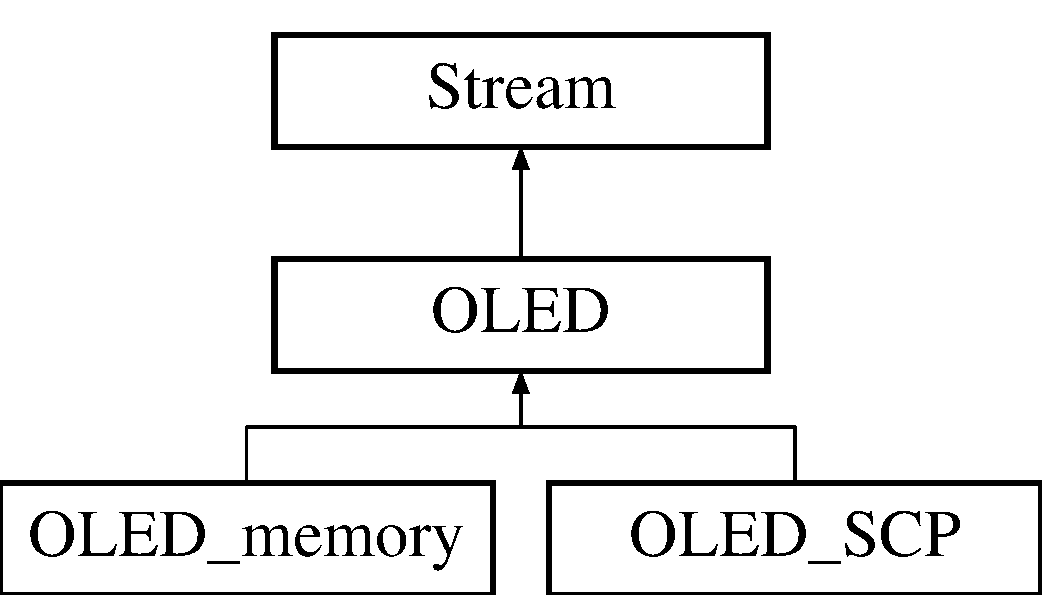
\includegraphics[height=3.000000cm]{class_o_l_e_d}
\end{center}
\end{figure}
\subsection*{Public Member Functions}
\begin{DoxyCompactItemize}
\item 
void \hyperlink{class_o_l_e_d_a2c8205c8eac9d7a2b181657561e9b4d2}{Init} (uint8\+\_\+t width, uint8\+\_\+t height)
\item 
void \hyperlink{class_o_l_e_d_a8d314130676b104ed959b92ab4bac25e}{Go\+To\+Line} (uint8\+\_\+t line)
\item 
void \hyperlink{class_o_l_e_d_a6c7bb1fc91b3e574a275f90643da140a}{Clear} ()
\item 
void \hyperlink{class_o_l_e_d_a3a571f5ea7a183fa14932cd5b2c423eb}{Clear\+Line} ()
\item 
void \hyperlink{class_o_l_e_d_a7fa307269dbd2e80a6e48a1442df83d2}{Write\+Byte} (uint8\+\_\+t page, uint8\+\_\+t column, uint8\+\_\+t byte)
\item 
void \hyperlink{class_o_l_e_d_a7fffc17a5439300d361414c15a7a2dbe}{Write\+Byte\+Array} (uint8\+\_\+t page, uint8\+\_\+t column, uint8\+\_\+t $\ast$byte\+\_\+array, uint8\+\_\+t length)
\item 
void \hyperlink{class_o_l_e_d_a3efa34861b4ae0bc5323f6b7cf1d8a01}{Repaint} ()
\item 
void \hyperlink{class_o_l_e_d_aa3c88e19f05340036ea5ac9e2d1ea5dc}{Set\+Number\+Of\+Lines} (uint8\+\_\+t \hyperlink{class_o_l_e_d_a9ea1c55112deede1a61142af276a6bc9}{number\+\_\+of\+\_\+lines})
\item 
void \hyperlink{class_o_l_e_d_a3cb468f16387343f6db387a86cded8af}{Write\+Bitmap} (uint8\+\_\+t $\ast$$\ast$pixels, uint8\+\_\+t bitmap\+\_\+width, uint8\+\_\+t bitmap\+\_\+height, uint8\+\_\+t x, uint8\+\_\+t y, bool is\+\_\+progmem)
\item 
void \hyperlink{class_o_l_e_d_abe6073c961cadc4c9b693eb8dc8198bd}{Set\+Font} (uint8\+\_\+t $\ast$\hyperlink{class_o_l_e_d_a29ab86a4a73f4d343bf1810927f0911d}{font}, uint8\+\_\+t width, uint8\+\_\+t height)
\item 
void \hyperlink{class_o_l_e_d_a0ffccb4fd874b997c869c5d511f76df8}{Write\+Line} (char $\ast$string, uint8\+\_\+t length, uint8\+\_\+t line, uint8\+\_\+t offset)
\item 
uint8\+\_\+t \hyperlink{class_o_l_e_d_a5b6d41d5d699998f54ea6e3b6562ac5b}{Get\+Y\+Coordinate\+From\+Line\+Number} (uint8\+\_\+t line)
\item 
uint8\+\_\+t \hyperlink{class_o_l_e_d_a7bb08915b685741c60bdccdd47781560}{Get\+Max\+Line\+Characters} ()
\end{DoxyCompactItemize}
\subsection*{Protected Member Functions}
\begin{DoxyCompactItemize}
\item 
\hyperlink{class_o_l_e_d_a8eabf371b5642d99800adb759dab27fd}{O\+L\+ED} ()
\item 
virtual void \hyperlink{class_o_l_e_d_a044fdff65656804114d1d39d766099a2}{Write\+Byte\+To\+O\+L\+ED} (volatile uint8\+\_\+t $\ast$address, uint8\+\_\+t data)
\item 
void \hyperlink{class_o_l_e_d_a3bd2f2f05568441e1e0533eaf0db58f8}{Get\+Bitmap\+For\+Character} (char character, uint8\+\_\+t $\ast$\&character\+\_\+bitmap)
\end{DoxyCompactItemize}
\subsection*{Protected Attributes}
\begin{DoxyCompactItemize}
\item 
uint8\+\_\+t \hyperlink{class_o_l_e_d_aebd62601be5e2ceef6295721f17fc013}{current\+\_\+line} = 0
\item 
uint8\+\_\+t \hyperlink{class_o_l_e_d_a2e9305cb3341509bb62d61f33cae76fd}{display\+\_\+width} = 0
\item 
uint8\+\_\+t \hyperlink{class_o_l_e_d_add08b51dec0ffeebcba7902c3bd4aeea}{display\+\_\+height} = 0
\item 
uint8\+\_\+t \hyperlink{class_o_l_e_d_aaac99b0eb4e9dfe92b8571488dc89288}{number\+\_\+of\+\_\+pages} = 0
\item 
uint8\+\_\+t \hyperlink{class_o_l_e_d_a9ea1c55112deede1a61142af276a6bc9}{number\+\_\+of\+\_\+lines} = 0
\item 
volatile uint8\+\_\+t $\ast$ \hyperlink{class_o_l_e_d_af0a85ccd0274347b8c1ac77d298a14cf}{oled\+\_\+command} = (volatile uint8\+\_\+t$\ast$)0x8000
\item 
volatile uint8\+\_\+t $\ast$ \hyperlink{class_o_l_e_d_a1bc54d49808f92ddfc354511b692df6f}{oled\+\_\+data} = (volatile uint8\+\_\+t$\ast$)0x8100
\item 
uint8\+\_\+t $\ast$$\ast$ \hyperlink{class_o_l_e_d_a9d32e21189940afba24deab0a2bc0126}{matrix}
\item 
uint8\+\_\+t \hyperlink{class_o_l_e_d_a6ddac7b826eccac8c682c5246ef52b29}{pixels\+\_\+per\+\_\+line}
\item 
uint8\+\_\+t $\ast$ \hyperlink{class_o_l_e_d_a29ab86a4a73f4d343bf1810927f0911d}{font} = nullptr
\item 
uint8\+\_\+t \hyperlink{class_o_l_e_d_a3c9ea103adf6c860a2534135e9a25ba8}{font\+\_\+width}
\item 
uint8\+\_\+t \hyperlink{class_o_l_e_d_a85b91421932866dea031921799ba83a3}{font\+\_\+height}
\end{DoxyCompactItemize}


\subsection{Detailed Description}
An interface to communicate with the \hyperlink{class_o_l_e_d}{O\+L\+ED} display. 

\subsection{Constructor \& Destructor Documentation}
\hypertarget{class_o_l_e_d_a8eabf371b5642d99800adb759dab27fd}{}\label{class_o_l_e_d_a8eabf371b5642d99800adb759dab27fd} 
\index{O\+L\+ED@{O\+L\+ED}!O\+L\+ED@{O\+L\+ED}}
\index{O\+L\+ED@{O\+L\+ED}!O\+L\+ED@{O\+L\+ED}}
\subsubsection{\texorpdfstring{O\+L\+E\+D()}{OLED()}}
{\footnotesize\ttfamily O\+L\+E\+D\+::\+O\+L\+ED (\begin{DoxyParamCaption}{ }\end{DoxyParamCaption})\hspace{0.3cm}{\ttfamily [protected]}}

Singleton constructor. 

\subsection{Member Function Documentation}
\hypertarget{class_o_l_e_d_a6c7bb1fc91b3e574a275f90643da140a}{}\label{class_o_l_e_d_a6c7bb1fc91b3e574a275f90643da140a} 
\index{O\+L\+ED@{O\+L\+ED}!Clear@{Clear}}
\index{Clear@{Clear}!O\+L\+ED@{O\+L\+ED}}
\subsubsection{\texorpdfstring{Clear()}{Clear()}}
{\footnotesize\ttfamily void O\+L\+E\+D\+::\+Clear (\begin{DoxyParamCaption}{ }\end{DoxyParamCaption})}

Clears the whole screen. \hypertarget{class_o_l_e_d_a3a571f5ea7a183fa14932cd5b2c423eb}{}\label{class_o_l_e_d_a3a571f5ea7a183fa14932cd5b2c423eb} 
\index{O\+L\+ED@{O\+L\+ED}!Clear\+Line@{Clear\+Line}}
\index{Clear\+Line@{Clear\+Line}!O\+L\+ED@{O\+L\+ED}}
\subsubsection{\texorpdfstring{Clear\+Line()}{ClearLine()}}
{\footnotesize\ttfamily void O\+L\+E\+D\+::\+Clear\+Line (\begin{DoxyParamCaption}{ }\end{DoxyParamCaption})}

Clears the current line. \hypertarget{class_o_l_e_d_a3bd2f2f05568441e1e0533eaf0db58f8}{}\label{class_o_l_e_d_a3bd2f2f05568441e1e0533eaf0db58f8} 
\index{O\+L\+ED@{O\+L\+ED}!Get\+Bitmap\+For\+Character@{Get\+Bitmap\+For\+Character}}
\index{Get\+Bitmap\+For\+Character@{Get\+Bitmap\+For\+Character}!O\+L\+ED@{O\+L\+ED}}
\subsubsection{\texorpdfstring{Get\+Bitmap\+For\+Character()}{GetBitmapForCharacter()}}
{\footnotesize\ttfamily void O\+L\+E\+D\+::\+Get\+Bitmap\+For\+Character (\begin{DoxyParamCaption}\item[{char}]{character,  }\item[{uint8\+\_\+t $\ast$\&}]{character\+\_\+bitmap }\end{DoxyParamCaption})\hspace{0.3cm}{\ttfamily [protected]}}

Fetches a pointer to P\+R\+O\+G\+M\+EM for the bitmap for the given font and character. Emphasis on that it points to P\+R\+O\+G\+M\+EM. \hypertarget{class_o_l_e_d_a7bb08915b685741c60bdccdd47781560}{}\label{class_o_l_e_d_a7bb08915b685741c60bdccdd47781560} 
\index{O\+L\+ED@{O\+L\+ED}!Get\+Max\+Line\+Characters@{Get\+Max\+Line\+Characters}}
\index{Get\+Max\+Line\+Characters@{Get\+Max\+Line\+Characters}!O\+L\+ED@{O\+L\+ED}}
\subsubsection{\texorpdfstring{Get\+Max\+Line\+Characters()}{GetMaxLineCharacters()}}
{\footnotesize\ttfamily uint8\+\_\+t O\+L\+E\+D\+::\+Get\+Max\+Line\+Characters (\begin{DoxyParamCaption}{ }\end{DoxyParamCaption})}

Returns how wide a line is in characters. \begin{DoxyReturn}{Returns}
How wide a line is in characters. 
\end{DoxyReturn}
\hypertarget{class_o_l_e_d_a5b6d41d5d699998f54ea6e3b6562ac5b}{}\label{class_o_l_e_d_a5b6d41d5d699998f54ea6e3b6562ac5b} 
\index{O\+L\+ED@{O\+L\+ED}!Get\+Y\+Coordinate\+From\+Line\+Number@{Get\+Y\+Coordinate\+From\+Line\+Number}}
\index{Get\+Y\+Coordinate\+From\+Line\+Number@{Get\+Y\+Coordinate\+From\+Line\+Number}!O\+L\+ED@{O\+L\+ED}}
\subsubsection{\texorpdfstring{Get\+Y\+Coordinate\+From\+Line\+Number()}{GetYCoordinateFromLineNumber()}}
{\footnotesize\ttfamily uint8\+\_\+t O\+L\+E\+D\+::\+Get\+Y\+Coordinate\+From\+Line\+Number (\begin{DoxyParamCaption}\item[{uint8\+\_\+t}]{line }\end{DoxyParamCaption})}

Returns the y coordinate of the line. 
\begin{DoxyParams}{Parameters}
{\em line} & The line to find the y coordinate of. \\
\hline
\end{DoxyParams}
\begin{DoxyReturn}{Returns}
The y coordinate of the line. 
\end{DoxyReturn}
\hypertarget{class_o_l_e_d_a8d314130676b104ed959b92ab4bac25e}{}\label{class_o_l_e_d_a8d314130676b104ed959b92ab4bac25e} 
\index{O\+L\+ED@{O\+L\+ED}!Go\+To\+Line@{Go\+To\+Line}}
\index{Go\+To\+Line@{Go\+To\+Line}!O\+L\+ED@{O\+L\+ED}}
\subsubsection{\texorpdfstring{Go\+To\+Line()}{GoToLine()}}
{\footnotesize\ttfamily void O\+L\+E\+D\+::\+Go\+To\+Line (\begin{DoxyParamCaption}\item[{uint8\+\_\+t}]{line }\end{DoxyParamCaption})}

Sets the line pointer. 
\begin{DoxyParams}{Parameters}
{\em line} & Which line to go to. \\
\hline
\end{DoxyParams}
\hypertarget{class_o_l_e_d_a2c8205c8eac9d7a2b181657561e9b4d2}{}\label{class_o_l_e_d_a2c8205c8eac9d7a2b181657561e9b4d2} 
\index{O\+L\+ED@{O\+L\+ED}!Init@{Init}}
\index{Init@{Init}!O\+L\+ED@{O\+L\+ED}}
\subsubsection{\texorpdfstring{Init()}{Init()}}
{\footnotesize\ttfamily void O\+L\+E\+D\+::\+Init (\begin{DoxyParamCaption}\item[{uint8\+\_\+t}]{width,  }\item[{uint8\+\_\+t}]{height }\end{DoxyParamCaption})}

Initializes the whole screen. 
\begin{DoxyParams}{Parameters}
{\em width} & The width of the screen in pixels. \\
\hline
{\em height} & The height of the screen in pixels. \\
\hline
\end{DoxyParams}
\hypertarget{class_o_l_e_d_a3efa34861b4ae0bc5323f6b7cf1d8a01}{}\label{class_o_l_e_d_a3efa34861b4ae0bc5323f6b7cf1d8a01} 
\index{O\+L\+ED@{O\+L\+ED}!Repaint@{Repaint}}
\index{Repaint@{Repaint}!O\+L\+ED@{O\+L\+ED}}
\subsubsection{\texorpdfstring{Repaint()}{Repaint()}}
{\footnotesize\ttfamily void O\+L\+E\+D\+::\+Repaint (\begin{DoxyParamCaption}{ }\end{DoxyParamCaption})}

Repaints the \hyperlink{class_o_l_e_d}{O\+L\+ED} \hypertarget{class_o_l_e_d_abe6073c961cadc4c9b693eb8dc8198bd}{}\label{class_o_l_e_d_abe6073c961cadc4c9b693eb8dc8198bd} 
\index{O\+L\+ED@{O\+L\+ED}!Set\+Font@{Set\+Font}}
\index{Set\+Font@{Set\+Font}!O\+L\+ED@{O\+L\+ED}}
\subsubsection{\texorpdfstring{Set\+Font()}{SetFont()}}
{\footnotesize\ttfamily void O\+L\+E\+D\+::\+Set\+Font (\begin{DoxyParamCaption}\item[{uint8\+\_\+t $\ast$}]{font,  }\item[{uint8\+\_\+t}]{width,  }\item[{uint8\+\_\+t}]{height }\end{DoxyParamCaption})}

Sets the font to be used when writing to the screen.


\begin{DoxyParams}{Parameters}
{\em font} & A pointer to the font. Put this on the P\+R\+O\+G\+M\+EM only if possible to save R\+AM space. \\
\hline
{\em width} & The width of the font in pixels. \\
\hline
{\em height} & The height of the font in pixels. \\
\hline
\end{DoxyParams}
\hypertarget{class_o_l_e_d_aa3c88e19f05340036ea5ac9e2d1ea5dc}{}\label{class_o_l_e_d_aa3c88e19f05340036ea5ac9e2d1ea5dc} 
\index{O\+L\+ED@{O\+L\+ED}!Set\+Number\+Of\+Lines@{Set\+Number\+Of\+Lines}}
\index{Set\+Number\+Of\+Lines@{Set\+Number\+Of\+Lines}!O\+L\+ED@{O\+L\+ED}}
\subsubsection{\texorpdfstring{Set\+Number\+Of\+Lines()}{SetNumberOfLines()}}
{\footnotesize\ttfamily void O\+L\+E\+D\+::\+Set\+Number\+Of\+Lines (\begin{DoxyParamCaption}\item[{uint8\+\_\+t}]{number\+\_\+of\+\_\+lines }\end{DoxyParamCaption})}

Sets the number of lines. Not to be confused with number of pages. 
\begin{DoxyParams}{Parameters}
{\em number\+\_\+of\+\_\+lines} & The number of lines. \\
\hline
\end{DoxyParams}
\hypertarget{class_o_l_e_d_a3cb468f16387343f6db387a86cded8af}{}\label{class_o_l_e_d_a3cb468f16387343f6db387a86cded8af} 
\index{O\+L\+ED@{O\+L\+ED}!Write\+Bitmap@{Write\+Bitmap}}
\index{Write\+Bitmap@{Write\+Bitmap}!O\+L\+ED@{O\+L\+ED}}
\subsubsection{\texorpdfstring{Write\+Bitmap()}{WriteBitmap()}}
{\footnotesize\ttfamily void O\+L\+E\+D\+::\+Write\+Bitmap (\begin{DoxyParamCaption}\item[{uint8\+\_\+t $\ast$$\ast$}]{pixels,  }\item[{uint8\+\_\+t}]{bitmap\+\_\+width,  }\item[{uint8\+\_\+t}]{bitmap\+\_\+height,  }\item[{uint8\+\_\+t}]{x,  }\item[{uint8\+\_\+t}]{y,  }\item[{bool}]{is\+\_\+progmem }\end{DoxyParamCaption})}

Writes a pixel matrix to the given x and y position on the display.


\begin{DoxyParams}{Parameters}
{\em pixels} & A double pointer to the matrix. \\
\hline
{\em bitmap\+\_\+width} & The width of the bitmap in pixels. \\
\hline
{\em bitmap\+\_\+height} & The height of the bitmap in pixels. \\
\hline
{\em x} & The starting position, x direction. \\
\hline
{\em y} & The starting position, y direction. \\
\hline
{\em is\+\_\+progmem} & A bool that indicates where the pixel array is located. \\
\hline
\end{DoxyParams}
\hypertarget{class_o_l_e_d_a7fa307269dbd2e80a6e48a1442df83d2}{}\label{class_o_l_e_d_a7fa307269dbd2e80a6e48a1442df83d2} 
\index{O\+L\+ED@{O\+L\+ED}!Write\+Byte@{Write\+Byte}}
\index{Write\+Byte@{Write\+Byte}!O\+L\+ED@{O\+L\+ED}}
\subsubsection{\texorpdfstring{Write\+Byte()}{WriteByte()}}
{\footnotesize\ttfamily void O\+L\+E\+D\+::\+Write\+Byte (\begin{DoxyParamCaption}\item[{uint8\+\_\+t}]{page,  }\item[{uint8\+\_\+t}]{column,  }\item[{uint8\+\_\+t}]{byte }\end{DoxyParamCaption})}

Writes a byte to the given page and column. This is a helper function mainly used for debugging. 
\begin{DoxyParams}{Parameters}
{\em page} & Which page to be written to. \\
\hline
{\em page} & Which column to be written to. \\
\hline
{\em byte} & The byte to be written. \\
\hline
\end{DoxyParams}
\hypertarget{class_o_l_e_d_a7fffc17a5439300d361414c15a7a2dbe}{}\label{class_o_l_e_d_a7fffc17a5439300d361414c15a7a2dbe} 
\index{O\+L\+ED@{O\+L\+ED}!Write\+Byte\+Array@{Write\+Byte\+Array}}
\index{Write\+Byte\+Array@{Write\+Byte\+Array}!O\+L\+ED@{O\+L\+ED}}
\subsubsection{\texorpdfstring{Write\+Byte\+Array()}{WriteByteArray()}}
{\footnotesize\ttfamily void O\+L\+E\+D\+::\+Write\+Byte\+Array (\begin{DoxyParamCaption}\item[{uint8\+\_\+t}]{page,  }\item[{uint8\+\_\+t}]{column,  }\item[{uint8\+\_\+t $\ast$}]{byte\+\_\+array,  }\item[{uint8\+\_\+t}]{length }\end{DoxyParamCaption})}

Writes a byte array starting at the given page and column. This is a helper function mainly used for debugging. 
\begin{DoxyParams}{Parameters}
{\em page} & Which page to be written to. \\
\hline
{\em page} & Which column to be written to first. \\
\hline
{\em byte\+\_\+array} & Bytes to be written. \\
\hline
{\em length} & The length of the byte array (number of columns). \\
\hline
\end{DoxyParams}
\hypertarget{class_o_l_e_d_a044fdff65656804114d1d39d766099a2}{}\label{class_o_l_e_d_a044fdff65656804114d1d39d766099a2} 
\index{O\+L\+ED@{O\+L\+ED}!Write\+Byte\+To\+O\+L\+ED@{Write\+Byte\+To\+O\+L\+ED}}
\index{Write\+Byte\+To\+O\+L\+ED@{Write\+Byte\+To\+O\+L\+ED}!O\+L\+ED@{O\+L\+ED}}
\subsubsection{\texorpdfstring{Write\+Byte\+To\+O\+L\+E\+D()}{WriteByteToOLED()}}
{\footnotesize\ttfamily virtual void O\+L\+E\+D\+::\+Write\+Byte\+To\+O\+L\+ED (\begin{DoxyParamCaption}\item[{volatile uint8\+\_\+t $\ast$}]{address,  }\item[{uint8\+\_\+t}]{data }\end{DoxyParamCaption})\hspace{0.3cm}{\ttfamily [inline]}, {\ttfamily [protected]}, {\ttfamily [virtual]}}

Writes a single byte to the \hyperlink{class_o_l_e_d}{O\+L\+ED}. This can be implemented using the external memory interface or using whatever other technology like for instance the \hyperlink{class_s_c_p}{S\+CP}. 
\begin{DoxyParams}{Parameters}
{\em address} & The address to write to. \\
\hline
{\em data} & The data to write. \\
\hline
\end{DoxyParams}


Reimplemented in \hyperlink{class_o_l_e_d___s_c_p_a5488fa5865fd8c0e83eb3c8ff7a216cf}{O\+L\+E\+D\+\_\+\+S\+CP}, and \hyperlink{class_o_l_e_d__memory_a8859cddd8c5639d43ae89bb750984291}{O\+L\+E\+D\+\_\+memory}.

\hypertarget{class_o_l_e_d_a0ffccb4fd874b997c869c5d511f76df8}{}\label{class_o_l_e_d_a0ffccb4fd874b997c869c5d511f76df8} 
\index{O\+L\+ED@{O\+L\+ED}!Write\+Line@{Write\+Line}}
\index{Write\+Line@{Write\+Line}!O\+L\+ED@{O\+L\+ED}}
\subsubsection{\texorpdfstring{Write\+Line()}{WriteLine()}}
{\footnotesize\ttfamily void O\+L\+E\+D\+::\+Write\+Line (\begin{DoxyParamCaption}\item[{char $\ast$}]{string,  }\item[{uint8\+\_\+t}]{length,  }\item[{uint8\+\_\+t}]{line,  }\item[{uint8\+\_\+t}]{offset }\end{DoxyParamCaption})}

Writes a string to the given line.


\begin{DoxyParams}{Parameters}
{\em string} & The string to be written. \\
\hline
{\em length} & Length of the string. \\
\hline
{\em line} & The line to write to. \\
\hline
{\em offset} & The offset from the left, in characters. \\
\hline
\end{DoxyParams}


\subsection{Member Data Documentation}
\hypertarget{class_o_l_e_d_aebd62601be5e2ceef6295721f17fc013}{}\label{class_o_l_e_d_aebd62601be5e2ceef6295721f17fc013} 
\index{O\+L\+ED@{O\+L\+ED}!current\+\_\+line@{current\+\_\+line}}
\index{current\+\_\+line@{current\+\_\+line}!O\+L\+ED@{O\+L\+ED}}
\subsubsection{\texorpdfstring{current\+\_\+line}{current\_line}}
{\footnotesize\ttfamily uint8\+\_\+t O\+L\+E\+D\+::current\+\_\+line = 0\hspace{0.3cm}{\ttfamily [protected]}}

The current line to write to. \hypertarget{class_o_l_e_d_add08b51dec0ffeebcba7902c3bd4aeea}{}\label{class_o_l_e_d_add08b51dec0ffeebcba7902c3bd4aeea} 
\index{O\+L\+ED@{O\+L\+ED}!display\+\_\+height@{display\+\_\+height}}
\index{display\+\_\+height@{display\+\_\+height}!O\+L\+ED@{O\+L\+ED}}
\subsubsection{\texorpdfstring{display\+\_\+height}{display\_height}}
{\footnotesize\ttfamily uint8\+\_\+t O\+L\+E\+D\+::display\+\_\+height = 0\hspace{0.3cm}{\ttfamily [protected]}}

Height of display in pixels. \hypertarget{class_o_l_e_d_a2e9305cb3341509bb62d61f33cae76fd}{}\label{class_o_l_e_d_a2e9305cb3341509bb62d61f33cae76fd} 
\index{O\+L\+ED@{O\+L\+ED}!display\+\_\+width@{display\+\_\+width}}
\index{display\+\_\+width@{display\+\_\+width}!O\+L\+ED@{O\+L\+ED}}
\subsubsection{\texorpdfstring{display\+\_\+width}{display\_width}}
{\footnotesize\ttfamily uint8\+\_\+t O\+L\+E\+D\+::display\+\_\+width = 0\hspace{0.3cm}{\ttfamily [protected]}}

Width of the display in pixels. \hypertarget{class_o_l_e_d_a29ab86a4a73f4d343bf1810927f0911d}{}\label{class_o_l_e_d_a29ab86a4a73f4d343bf1810927f0911d} 
\index{O\+L\+ED@{O\+L\+ED}!font@{font}}
\index{font@{font}!O\+L\+ED@{O\+L\+ED}}
\subsubsection{\texorpdfstring{font}{font}}
{\footnotesize\ttfamily uint8\+\_\+t$\ast$ O\+L\+E\+D\+::font = nullptr\hspace{0.3cm}{\ttfamily [protected]}}

The font to use for writing. \hypertarget{class_o_l_e_d_a85b91421932866dea031921799ba83a3}{}\label{class_o_l_e_d_a85b91421932866dea031921799ba83a3} 
\index{O\+L\+ED@{O\+L\+ED}!font\+\_\+height@{font\+\_\+height}}
\index{font\+\_\+height@{font\+\_\+height}!O\+L\+ED@{O\+L\+ED}}
\subsubsection{\texorpdfstring{font\+\_\+height}{font\_height}}
{\footnotesize\ttfamily uint8\+\_\+t O\+L\+E\+D\+::font\+\_\+height\hspace{0.3cm}{\ttfamily [protected]}}

Height of the font in pixels. \hypertarget{class_o_l_e_d_a3c9ea103adf6c860a2534135e9a25ba8}{}\label{class_o_l_e_d_a3c9ea103adf6c860a2534135e9a25ba8} 
\index{O\+L\+ED@{O\+L\+ED}!font\+\_\+width@{font\+\_\+width}}
\index{font\+\_\+width@{font\+\_\+width}!O\+L\+ED@{O\+L\+ED}}
\subsubsection{\texorpdfstring{font\+\_\+width}{font\_width}}
{\footnotesize\ttfamily uint8\+\_\+t O\+L\+E\+D\+::font\+\_\+width\hspace{0.3cm}{\ttfamily [protected]}}

Width of the font in pixels. \hypertarget{class_o_l_e_d_a9d32e21189940afba24deab0a2bc0126}{}\label{class_o_l_e_d_a9d32e21189940afba24deab0a2bc0126} 
\index{O\+L\+ED@{O\+L\+ED}!matrix@{matrix}}
\index{matrix@{matrix}!O\+L\+ED@{O\+L\+ED}}
\subsubsection{\texorpdfstring{matrix}{matrix}}
{\footnotesize\ttfamily uint8\+\_\+t$\ast$$\ast$ O\+L\+E\+D\+::matrix\hspace{0.3cm}{\ttfamily [protected]}}

The display buffer. There is also a buffer on the \hyperlink{class_o_l_e_d}{O\+L\+ED} controller, such that this implements a dual buffer. \hypertarget{class_o_l_e_d_a9ea1c55112deede1a61142af276a6bc9}{}\label{class_o_l_e_d_a9ea1c55112deede1a61142af276a6bc9} 
\index{O\+L\+ED@{O\+L\+ED}!number\+\_\+of\+\_\+lines@{number\+\_\+of\+\_\+lines}}
\index{number\+\_\+of\+\_\+lines@{number\+\_\+of\+\_\+lines}!O\+L\+ED@{O\+L\+ED}}
\subsubsection{\texorpdfstring{number\+\_\+of\+\_\+lines}{number\_of\_lines}}
{\footnotesize\ttfamily uint8\+\_\+t O\+L\+E\+D\+::number\+\_\+of\+\_\+lines = 0\hspace{0.3cm}{\ttfamily [protected]}}

Number of lines. Not to be confused with number of pages. \hypertarget{class_o_l_e_d_aaac99b0eb4e9dfe92b8571488dc89288}{}\label{class_o_l_e_d_aaac99b0eb4e9dfe92b8571488dc89288} 
\index{O\+L\+ED@{O\+L\+ED}!number\+\_\+of\+\_\+pages@{number\+\_\+of\+\_\+pages}}
\index{number\+\_\+of\+\_\+pages@{number\+\_\+of\+\_\+pages}!O\+L\+ED@{O\+L\+ED}}
\subsubsection{\texorpdfstring{number\+\_\+of\+\_\+pages}{number\_of\_pages}}
{\footnotesize\ttfamily uint8\+\_\+t O\+L\+E\+D\+::number\+\_\+of\+\_\+pages = 0\hspace{0.3cm}{\ttfamily [protected]}}

Number of pages \hypertarget{class_o_l_e_d_af0a85ccd0274347b8c1ac77d298a14cf}{}\label{class_o_l_e_d_af0a85ccd0274347b8c1ac77d298a14cf} 
\index{O\+L\+ED@{O\+L\+ED}!oled\+\_\+command@{oled\+\_\+command}}
\index{oled\+\_\+command@{oled\+\_\+command}!O\+L\+ED@{O\+L\+ED}}
\subsubsection{\texorpdfstring{oled\+\_\+command}{oled\_command}}
{\footnotesize\ttfamily volatile uint8\+\_\+t$\ast$ O\+L\+E\+D\+::oled\+\_\+command = (volatile uint8\+\_\+t$\ast$)0x8000\hspace{0.3cm}{\ttfamily [protected]}}

A pointer to where the O\+L\+E\+D\+\_\+\+C\+O\+M\+M\+A\+ND address space starts. \hypertarget{class_o_l_e_d_a1bc54d49808f92ddfc354511b692df6f}{}\label{class_o_l_e_d_a1bc54d49808f92ddfc354511b692df6f} 
\index{O\+L\+ED@{O\+L\+ED}!oled\+\_\+data@{oled\+\_\+data}}
\index{oled\+\_\+data@{oled\+\_\+data}!O\+L\+ED@{O\+L\+ED}}
\subsubsection{\texorpdfstring{oled\+\_\+data}{oled\_data}}
{\footnotesize\ttfamily volatile uint8\+\_\+t$\ast$ O\+L\+E\+D\+::oled\+\_\+data = (volatile uint8\+\_\+t$\ast$)0x8100\hspace{0.3cm}{\ttfamily [protected]}}

A pointer to where the O\+L\+E\+D\+\_\+\+D\+A\+TA address space starts. \hypertarget{class_o_l_e_d_a6ddac7b826eccac8c682c5246ef52b29}{}\label{class_o_l_e_d_a6ddac7b826eccac8c682c5246ef52b29} 
\index{O\+L\+ED@{O\+L\+ED}!pixels\+\_\+per\+\_\+line@{pixels\+\_\+per\+\_\+line}}
\index{pixels\+\_\+per\+\_\+line@{pixels\+\_\+per\+\_\+line}!O\+L\+ED@{O\+L\+ED}}
\subsubsection{\texorpdfstring{pixels\+\_\+per\+\_\+line}{pixels\_per\_line}}
{\footnotesize\ttfamily uint8\+\_\+t O\+L\+E\+D\+::pixels\+\_\+per\+\_\+line\hspace{0.3cm}{\ttfamily [protected]}}

The number of pixels per line. 

The documentation for this class was generated from the following files\+:\begin{DoxyCompactItemize}
\item 
lib/oled/oled.\+h\item 
lib/oled/oled.\+cpp\end{DoxyCompactItemize}

\hypertarget{class_stream}{\section{Stream Class Reference}
\label{class_stream}\index{Stream@{Stream}}
}
Inheritance diagram for Stream\-:\begin{figure}[H]
\begin{center}
\leavevmode
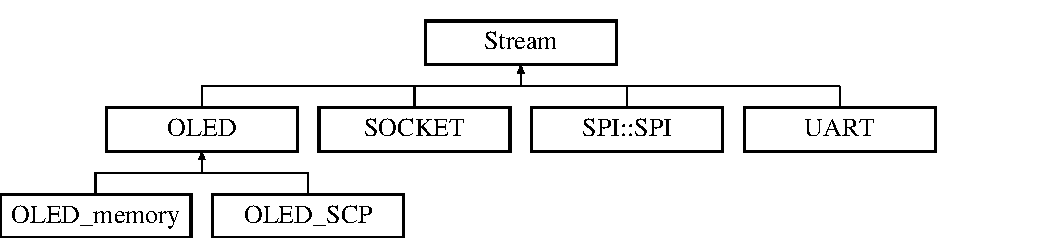
\includegraphics[height=2.000000cm]{class_stream}
\end{center}
\end{figure}
\subsection*{Public Member Functions}
\begin{DoxyCompactItemize}
\item 
\hyperlink{class_stream_afd83bbd749c467ad3dd85e1b80170c9b}{Stream} (uint8\-\_\-t $\ast$\hyperlink{class_stream_aaa6b266a85844345faee432d0267c6ec}{input\-\_\-stream}, uint16\-\_\-t \hyperlink{class_stream_a8a754b0acc9552d1b78de92b2476f4cb}{input\-\_\-stream\-\_\-size}, uint8\-\_\-t $\ast$\hyperlink{class_stream_ab2d136f405b24e5eb2a6058b24fabfa3}{output\-\_\-stream}, uint16\-\_\-t \hyperlink{class_stream_a3a171d646ab70eeb9c034aecb3a72003}{output\-\_\-stream\-\_\-size})
\item 
virtual void \hyperlink{class_stream_a508be3423e4d99ab2757275fb723002a}{Write} (uint8\-\_\-t $\ast$string, uint16\-\_\-t size)
\item 
virtual void \hyperlink{class_stream_a4f3ec0f7a24ddcfd054566feb614afba}{Read} (uint8\-\_\-t $\ast$string, uint16\-\_\-t size)
\item 
virtual uint8\-\_\-t \hyperlink{class_stream_aeb3f1b3d55f4b502c02d73ce4de42714}{Read\-Byte} ()
\item 
virtual void \hyperlink{class_stream_aeaed767b3a8d946c6f81465fa83ff17f}{Write\-Byte} (uint8\-\_\-t byte)
\item 
virtual uint8\-\_\-t \hyperlink{class_stream_a6a16ddb03d3360cef4daf4d38245091d}{Get\-Available\-Write\-Bytes} ()
\item 
virtual uint8\-\_\-t \hyperlink{class_stream_a71cec6c46f3d50cc3ab420e93ae434e1}{Get\-Available\-Read\-Bytes} ()
\item 
virtual bool \hyperlink{class_stream_a088c4e68d568acfad715c56f408fe9f8}{Check\-Input\-Overflow\-Flag} ()
\item 
virtual bool \hyperlink{class_stream_aee6c201819b874c5934a270592d9d311}{Check\-Output\-Overflow\-Flag} ()
\end{DoxyCompactItemize}
\subsection*{Protected Member Functions}
\begin{DoxyCompactItemize}
\item 
virtual void \hyperlink{class_stream_add5927208d603b08341f8972652d9c44}{Read\-From\-Buffer} (uint8\-\_\-t $\ast$buffer, uint16\-\_\-t \&start\-\_\-index, uint16\-\_\-t \&stop\-\_\-index, uint16\-\_\-t \&buffer\-\_\-size, uint8\-\_\-t $\ast$string, uint16\-\_\-t \&string\-\_\-size)
\item 
virtual void \hyperlink{class_stream_a456d59b1944143a8e4a977b8861d42ea}{Write\-To\-Buffer} (uint8\-\_\-t $\ast$buffer, uint16\-\_\-t \&start\-\_\-index, uint16\-\_\-t \&stop\-\_\-index, uint16\-\_\-t \&buffer\-\_\-size, bool \&overflow\-\_\-flag, uint8\-\_\-t $\ast$string, uint16\-\_\-t \&string\-\_\-size)
\item 
virtual uint8\-\_\-t \hyperlink{class_stream_a6c49bb8565d238e13c3ca3e9eddcf38e}{Read\-Byte\-From\-Buffer} (uint8\-\_\-t $\ast$buffer, uint16\-\_\-t \&start\-\_\-index, uint16\-\_\-t \&stop\-\_\-index, uint16\-\_\-t \&buffer\-\_\-size)
\item 
virtual void \hyperlink{class_stream_a129f3c3e763ceab692bdde38fdc89402}{Write\-Byte\-To\-Buffer} (uint8\-\_\-t $\ast$buffer, uint16\-\_\-t \&start\-\_\-index, uint16\-\_\-t \&stop\-\_\-index, uint16\-\_\-t \&buffer\-\_\-size, bool \&overflow\-\_\-flag, uint8\-\_\-t \&byte)
\item 
virtual void \hyperlink{class_stream_a70108ab0e811c6cab2636bf7afeb5e14}{Write\-Byte\-To\-Input\-Stream} (uint8\-\_\-t byte)
\item 
virtual uint8\-\_\-t \hyperlink{class_stream_a712a8e0c6659799b1bb2999b53bd983d}{Read\-Byte\-From\-Output\-Stream} ()
\item 
virtual void \hyperlink{class_stream_aa2f020721d273ce821ccf626e5eb773c}{Write\-To\-Input\-Stream} (uint8\-\_\-t $\ast$string, uint16\-\_\-t size)
\item 
virtual void \hyperlink{class_stream_adce437b86a098710237ac7dcccd5508d}{Read\-From\-Output\-Stream} (uint8\-\_\-t $\ast$string, uint16\-\_\-t size)
\item 
virtual uint16\-\_\-t \hyperlink{class_stream_a8abdeaae6339d9873842a951843cb386}{Calculate\-Length} (uint16\-\_\-t \&start\-\_\-index, uint16\-\_\-t \&stop\-\_\-index, uint16\-\_\-t \&buffer\-\_\-size)
\item 
virtual uint16\-\_\-t \hyperlink{class_stream_ac9d4705ce8fe5c9ac473939fcac423f6}{Get\-Input\-Stream\-Length} ()
\item 
virtual uint16\-\_\-t \hyperlink{class_stream_a6378bb812d0b77890926d1c724140146}{Get\-Output\-Stream\-Length} ()
\end{DoxyCompactItemize}
\subsection*{Protected Attributes}
\begin{DoxyCompactItemize}
\item 
uint8\-\_\-t $\ast$ \hyperlink{class_stream_aaa6b266a85844345faee432d0267c6ec}{input\-\_\-stream} = nullptr
\item 
uint8\-\_\-t $\ast$ \hyperlink{class_stream_ab2d136f405b24e5eb2a6058b24fabfa3}{output\-\_\-stream} = nullptr
\item 
uint16\-\_\-t \hyperlink{class_stream_ade2d5afb993214626e7c7d66cb76cd46}{input\-\_\-stream\-\_\-start\-\_\-index} = 0
\item 
uint16\-\_\-t \hyperlink{class_stream_a7406f5db92c18f0a6d7dcc924a6122cc}{output\-\_\-stream\-\_\-start\-\_\-index} = 0
\item 
uint16\-\_\-t \hyperlink{class_stream_a52cf2f675dd7ec342615e82cc29513de}{input\-\_\-stream\-\_\-stop\-\_\-index} = 0
\item 
uint16\-\_\-t \hyperlink{class_stream_ac3b2282b5977151124aa77c2d4e411ec}{output\-\_\-stream\-\_\-stop\-\_\-index} = 0
\item 
uint16\-\_\-t \hyperlink{class_stream_a3a171d646ab70eeb9c034aecb3a72003}{output\-\_\-stream\-\_\-size} = 0
\item 
uint16\-\_\-t \hyperlink{class_stream_a8a754b0acc9552d1b78de92b2476f4cb}{input\-\_\-stream\-\_\-size} = 0
\item 
bool \hyperlink{class_stream_aeffd88d8ca71bf0d084ded2a251e3a57}{input\-\_\-stream\-\_\-overflowed} = false
\item 
bool \hyperlink{class_stream_a91eb40b21c46bd57b61811a890ac047a}{output\-\_\-stream\-\_\-overflowed} = false
\end{DoxyCompactItemize}


\subsection{Constructor \& Destructor Documentation}
\hypertarget{class_stream_afd83bbd749c467ad3dd85e1b80170c9b}{\index{Stream@{Stream}!Stream@{Stream}}
\index{Stream@{Stream}!Stream@{Stream}}
\subsubsection[{Stream}]{\setlength{\rightskip}{0pt plus 5cm}Stream\-::\-Stream (
\begin{DoxyParamCaption}
\item[{uint8\-\_\-t $\ast$}]{input\-\_\-stream, }
\item[{uint16\-\_\-t}]{input\-\_\-stream\-\_\-size, }
\item[{uint8\-\_\-t $\ast$}]{output\-\_\-stream, }
\item[{uint16\-\_\-t}]{output\-\_\-stream\-\_\-size}
\end{DoxyParamCaption}
)\hspace{0.3cm}{\ttfamily [inline]}}}\label{class_stream_afd83bbd749c467ad3dd85e1b80170c9b}
The constructor. Needed to initialize stream sizes 
\begin{DoxyParams}{Parameters}
{\em input\-\_\-stream\-\_\-size} & The size of the input ring buffer. \\
\hline
{\em output\-\_\-stream\-\_\-size} & The size of the output ring buffer. \\
\hline
\end{DoxyParams}


\subsection{Member Function Documentation}
\hypertarget{class_stream_a8abdeaae6339d9873842a951843cb386}{\index{Stream@{Stream}!Calculate\-Length@{Calculate\-Length}}
\index{Calculate\-Length@{Calculate\-Length}!Stream@{Stream}}
\subsubsection[{Calculate\-Length}]{\setlength{\rightskip}{0pt plus 5cm}uint16\-\_\-t Stream\-::\-Calculate\-Length (
\begin{DoxyParamCaption}
\item[{uint16\-\_\-t \&}]{start\-\_\-index, }
\item[{uint16\-\_\-t \&}]{stop\-\_\-index, }
\item[{uint16\-\_\-t \&}]{buffer\-\_\-size}
\end{DoxyParamCaption}
)\hspace{0.3cm}{\ttfamily [protected]}, {\ttfamily [virtual]}}}\label{class_stream_a8abdeaae6339d9873842a951843cb386}
Calculates the length of the readable part of the buffer 
\begin{DoxyParams}{Parameters}
{\em start\-\_\-index} & The start index of the buffer \\
\hline
{\em stop\-\_\-index} & The stop index of the buffer \\
\hline
\end{DoxyParams}
\begin{DoxyReturn}{Returns}
Length of valid data 
\end{DoxyReturn}
\hypertarget{class_stream_a088c4e68d568acfad715c56f408fe9f8}{\index{Stream@{Stream}!Check\-Input\-Overflow\-Flag@{Check\-Input\-Overflow\-Flag}}
\index{Check\-Input\-Overflow\-Flag@{Check\-Input\-Overflow\-Flag}!Stream@{Stream}}
\subsubsection[{Check\-Input\-Overflow\-Flag}]{\setlength{\rightskip}{0pt plus 5cm}bool Stream\-::\-Check\-Input\-Overflow\-Flag (
\begin{DoxyParamCaption}
{}
\end{DoxyParamCaption}
)\hspace{0.3cm}{\ttfamily [virtual]}}}\label{class_stream_a088c4e68d568acfad715c56f408fe9f8}
Checks whether or not the input overflow flag has been set. If it has, it conducts the nessesary procedures to clear out the overflow \hypertarget{class_stream_aee6c201819b874c5934a270592d9d311}{\index{Stream@{Stream}!Check\-Output\-Overflow\-Flag@{Check\-Output\-Overflow\-Flag}}
\index{Check\-Output\-Overflow\-Flag@{Check\-Output\-Overflow\-Flag}!Stream@{Stream}}
\subsubsection[{Check\-Output\-Overflow\-Flag}]{\setlength{\rightskip}{0pt plus 5cm}bool Stream\-::\-Check\-Output\-Overflow\-Flag (
\begin{DoxyParamCaption}
{}
\end{DoxyParamCaption}
)\hspace{0.3cm}{\ttfamily [virtual]}}}\label{class_stream_aee6c201819b874c5934a270592d9d311}
Checks whether or not the output overflow flag has been set. If it has, it conducts the nessesary procedures to clear out the overflow \hypertarget{class_stream_a71cec6c46f3d50cc3ab420e93ae434e1}{\index{Stream@{Stream}!Get\-Available\-Read\-Bytes@{Get\-Available\-Read\-Bytes}}
\index{Get\-Available\-Read\-Bytes@{Get\-Available\-Read\-Bytes}!Stream@{Stream}}
\subsubsection[{Get\-Available\-Read\-Bytes}]{\setlength{\rightskip}{0pt plus 5cm}uint8\-\_\-t Stream\-::\-Get\-Available\-Read\-Bytes (
\begin{DoxyParamCaption}
{}
\end{DoxyParamCaption}
)\hspace{0.3cm}{\ttfamily [virtual]}}}\label{class_stream_a71cec6c46f3d50cc3ab420e93ae434e1}
Simply returns the number of bytes available for reading (the actual data available for receiving in the buffer) \hypertarget{class_stream_a6a16ddb03d3360cef4daf4d38245091d}{\index{Stream@{Stream}!Get\-Available\-Write\-Bytes@{Get\-Available\-Write\-Bytes}}
\index{Get\-Available\-Write\-Bytes@{Get\-Available\-Write\-Bytes}!Stream@{Stream}}
\subsubsection[{Get\-Available\-Write\-Bytes}]{\setlength{\rightskip}{0pt plus 5cm}uint8\-\_\-t Stream\-::\-Get\-Available\-Write\-Bytes (
\begin{DoxyParamCaption}
{}
\end{DoxyParamCaption}
)\hspace{0.3cm}{\ttfamily [virtual]}}}\label{class_stream_a6a16ddb03d3360cef4daf4d38245091d}
Simply returns the number of bytes available in the output buffer. The output depends on the maximum bytes allocated in the implementation. \hypertarget{class_stream_ac9d4705ce8fe5c9ac473939fcac423f6}{\index{Stream@{Stream}!Get\-Input\-Stream\-Length@{Get\-Input\-Stream\-Length}}
\index{Get\-Input\-Stream\-Length@{Get\-Input\-Stream\-Length}!Stream@{Stream}}
\subsubsection[{Get\-Input\-Stream\-Length}]{\setlength{\rightskip}{0pt plus 5cm}uint16\-\_\-t Stream\-::\-Get\-Input\-Stream\-Length (
\begin{DoxyParamCaption}
{}
\end{DoxyParamCaption}
)\hspace{0.3cm}{\ttfamily [protected]}, {\ttfamily [virtual]}}}\label{class_stream_ac9d4705ce8fe5c9ac473939fcac423f6}
Calculates the length of the readable part of the buffer 
\begin{DoxyParams}{Parameters}
{\em start\-\_\-index} & The start index of the buffer \\
\hline
{\em stop\-\_\-index} & The stop index of the buffer \\
\hline
\end{DoxyParams}
\begin{DoxyReturn}{Returns}
Length of valid data 
\end{DoxyReturn}
\hypertarget{class_stream_a6378bb812d0b77890926d1c724140146}{\index{Stream@{Stream}!Get\-Output\-Stream\-Length@{Get\-Output\-Stream\-Length}}
\index{Get\-Output\-Stream\-Length@{Get\-Output\-Stream\-Length}!Stream@{Stream}}
\subsubsection[{Get\-Output\-Stream\-Length}]{\setlength{\rightskip}{0pt plus 5cm}uint16\-\_\-t Stream\-::\-Get\-Output\-Stream\-Length (
\begin{DoxyParamCaption}
{}
\end{DoxyParamCaption}
)\hspace{0.3cm}{\ttfamily [protected]}, {\ttfamily [virtual]}}}\label{class_stream_a6378bb812d0b77890926d1c724140146}
Calculates the length of the readable part of the buffer \begin{DoxyReturn}{Returns}
Length of valid data 
\end{DoxyReturn}
\hypertarget{class_stream_a4f3ec0f7a24ddcfd054566feb614afba}{\index{Stream@{Stream}!Read@{Read}}
\index{Read@{Read}!Stream@{Stream}}
\subsubsection[{Read}]{\setlength{\rightskip}{0pt plus 5cm}void Stream\-::\-Read (
\begin{DoxyParamCaption}
\item[{uint8\-\_\-t $\ast$}]{string, }
\item[{uint16\-\_\-t}]{size}
\end{DoxyParamCaption}
)\hspace{0.3cm}{\ttfamily [virtual]}}}\label{class_stream_a4f3ec0f7a24ddcfd054566feb614afba}
Reads data from the input stream and stores in the specified data. 
\begin{DoxyParams}{Parameters}
{\em string} & Where the data should be stored \\
\hline
{\em size} & Size of the data \\
\hline
\end{DoxyParams}
\hypertarget{class_stream_aeb3f1b3d55f4b502c02d73ce4de42714}{\index{Stream@{Stream}!Read\-Byte@{Read\-Byte}}
\index{Read\-Byte@{Read\-Byte}!Stream@{Stream}}
\subsubsection[{Read\-Byte}]{\setlength{\rightskip}{0pt plus 5cm}uint8\-\_\-t Stream\-::\-Read\-Byte (
\begin{DoxyParamCaption}
{}
\end{DoxyParamCaption}
)\hspace{0.3cm}{\ttfamily [virtual]}}}\label{class_stream_aeb3f1b3d55f4b502c02d73ce4de42714}
Reads one byte from the input stream \hypertarget{class_stream_a6c49bb8565d238e13c3ca3e9eddcf38e}{\index{Stream@{Stream}!Read\-Byte\-From\-Buffer@{Read\-Byte\-From\-Buffer}}
\index{Read\-Byte\-From\-Buffer@{Read\-Byte\-From\-Buffer}!Stream@{Stream}}
\subsubsection[{Read\-Byte\-From\-Buffer}]{\setlength{\rightskip}{0pt plus 5cm}uint8\-\_\-t Stream\-::\-Read\-Byte\-From\-Buffer (
\begin{DoxyParamCaption}
\item[{uint8\-\_\-t $\ast$}]{buffer, }
\item[{uint16\-\_\-t \&}]{start\-\_\-index, }
\item[{uint16\-\_\-t \&}]{stop\-\_\-index, }
\item[{uint16\-\_\-t \&}]{buffer\-\_\-size}
\end{DoxyParamCaption}
)\hspace{0.3cm}{\ttfamily [protected]}, {\ttfamily [virtual]}}}\label{class_stream_a6c49bb8565d238e13c3ca3e9eddcf38e}
Reads a byte from the given buffer 
\begin{DoxyParams}{Parameters}
{\em buffer} & The buffer to read from \\
\hline
{\em start\-\_\-index} & The first valid bit of the buffer \\
\hline
{\em stop\-\_\-index} & The last valid bit of the buffer \\
\hline
{\em size} & The size of the buffer \\
\hline
\end{DoxyParams}
\begin{DoxyReturn}{Returns}
The byte that was read 
\end{DoxyReturn}
\hypertarget{class_stream_a712a8e0c6659799b1bb2999b53bd983d}{\index{Stream@{Stream}!Read\-Byte\-From\-Output\-Stream@{Read\-Byte\-From\-Output\-Stream}}
\index{Read\-Byte\-From\-Output\-Stream@{Read\-Byte\-From\-Output\-Stream}!Stream@{Stream}}
\subsubsection[{Read\-Byte\-From\-Output\-Stream}]{\setlength{\rightskip}{0pt plus 5cm}uint8\-\_\-t Stream\-::\-Read\-Byte\-From\-Output\-Stream (
\begin{DoxyParamCaption}
{}
\end{DoxyParamCaption}
)\hspace{0.3cm}{\ttfamily [protected]}, {\ttfamily [virtual]}}}\label{class_stream_a712a8e0c6659799b1bb2999b53bd983d}
Reads a byte from the output stream \hypertarget{class_stream_add5927208d603b08341f8972652d9c44}{\index{Stream@{Stream}!Read\-From\-Buffer@{Read\-From\-Buffer}}
\index{Read\-From\-Buffer@{Read\-From\-Buffer}!Stream@{Stream}}
\subsubsection[{Read\-From\-Buffer}]{\setlength{\rightskip}{0pt plus 5cm}void Stream\-::\-Read\-From\-Buffer (
\begin{DoxyParamCaption}
\item[{uint8\-\_\-t $\ast$}]{buffer, }
\item[{uint16\-\_\-t \&}]{start\-\_\-index, }
\item[{uint16\-\_\-t \&}]{stop\-\_\-index, }
\item[{uint16\-\_\-t \&}]{buffer\-\_\-size, }
\item[{uint8\-\_\-t $\ast$}]{string, }
\item[{uint16\-\_\-t \&}]{string\-\_\-size}
\end{DoxyParamCaption}
)\hspace{0.3cm}{\ttfamily [protected]}, {\ttfamily [virtual]}}}\label{class_stream_add5927208d603b08341f8972652d9c44}
Reads a string from the given buffer. 
\begin{DoxyParams}{Parameters}
{\em buffer} & Buffer to read from \\
\hline
{\em start\-\_\-index} & The first valid byte of the buffer \\
\hline
{\em stop\-\_\-index} & The last valid byte of the buffer \\
\hline
{\em size} & The size of the buffer \\
\hline
{\em string} & The string to read into \\
\hline
{\em length} & The length of the string \\
\hline
\end{DoxyParams}
\hypertarget{class_stream_adce437b86a098710237ac7dcccd5508d}{\index{Stream@{Stream}!Read\-From\-Output\-Stream@{Read\-From\-Output\-Stream}}
\index{Read\-From\-Output\-Stream@{Read\-From\-Output\-Stream}!Stream@{Stream}}
\subsubsection[{Read\-From\-Output\-Stream}]{\setlength{\rightskip}{0pt plus 5cm}void Stream\-::\-Read\-From\-Output\-Stream (
\begin{DoxyParamCaption}
\item[{uint8\-\_\-t $\ast$}]{string, }
\item[{uint16\-\_\-t}]{size}
\end{DoxyParamCaption}
)\hspace{0.3cm}{\ttfamily [protected]}, {\ttfamily [virtual]}}}\label{class_stream_adce437b86a098710237ac7dcccd5508d}
Reads data from the input stream and stores in the specified data. 
\begin{DoxyParams}{Parameters}
{\em string} & Where the data should be stored \\
\hline
{\em size} & Size of the data \\
\hline
\end{DoxyParams}
\hypertarget{class_stream_a508be3423e4d99ab2757275fb723002a}{\index{Stream@{Stream}!Write@{Write}}
\index{Write@{Write}!Stream@{Stream}}
\subsubsection[{Write}]{\setlength{\rightskip}{0pt plus 5cm}void Stream\-::\-Write (
\begin{DoxyParamCaption}
\item[{uint8\-\_\-t $\ast$}]{string, }
\item[{uint16\-\_\-t}]{size}
\end{DoxyParamCaption}
)\hspace{0.3cm}{\ttfamily [virtual]}}}\label{class_stream_a508be3423e4d99ab2757275fb723002a}
Writes the specified data to the output stream. 
\begin{DoxyParams}{Parameters}
{\em string} & Input data \\
\hline
{\em size} & Size of the input data \\
\hline
\end{DoxyParams}
\hypertarget{class_stream_aeaed767b3a8d946c6f81465fa83ff17f}{\index{Stream@{Stream}!Write\-Byte@{Write\-Byte}}
\index{Write\-Byte@{Write\-Byte}!Stream@{Stream}}
\subsubsection[{Write\-Byte}]{\setlength{\rightskip}{0pt plus 5cm}void Stream\-::\-Write\-Byte (
\begin{DoxyParamCaption}
\item[{uint8\-\_\-t}]{byte}
\end{DoxyParamCaption}
)\hspace{0.3cm}{\ttfamily [virtual]}}}\label{class_stream_aeaed767b3a8d946c6f81465fa83ff17f}
Writes one byte to the output stream \hypertarget{class_stream_a129f3c3e763ceab692bdde38fdc89402}{\index{Stream@{Stream}!Write\-Byte\-To\-Buffer@{Write\-Byte\-To\-Buffer}}
\index{Write\-Byte\-To\-Buffer@{Write\-Byte\-To\-Buffer}!Stream@{Stream}}
\subsubsection[{Write\-Byte\-To\-Buffer}]{\setlength{\rightskip}{0pt plus 5cm}void Stream\-::\-Write\-Byte\-To\-Buffer (
\begin{DoxyParamCaption}
\item[{uint8\-\_\-t $\ast$}]{buffer, }
\item[{uint16\-\_\-t \&}]{start\-\_\-index, }
\item[{uint16\-\_\-t \&}]{stop\-\_\-index, }
\item[{uint16\-\_\-t \&}]{buffer\-\_\-size, }
\item[{bool \&}]{overflow\-\_\-flag, }
\item[{uint8\-\_\-t \&}]{byte}
\end{DoxyParamCaption}
)\hspace{0.3cm}{\ttfamily [protected]}, {\ttfamily [virtual]}}}\label{class_stream_a129f3c3e763ceab692bdde38fdc89402}
Writes a byte to the buffer 
\begin{DoxyParams}{Parameters}
{\em buffer} & The buffer to write to \\
\hline
{\em start\-\_\-index} & The first valid bit of the buffer \\
\hline
{\em stop\-\_\-index} & The last valid bit of the buffer \\
\hline
{\em size} & The size of the buffer \\
\hline
{\em byte} & The byte to be written \\
\hline
{\em overflow\-\_\-flag} & A flag indicated an overflow \\
\hline
\end{DoxyParams}
\hypertarget{class_stream_a70108ab0e811c6cab2636bf7afeb5e14}{\index{Stream@{Stream}!Write\-Byte\-To\-Input\-Stream@{Write\-Byte\-To\-Input\-Stream}}
\index{Write\-Byte\-To\-Input\-Stream@{Write\-Byte\-To\-Input\-Stream}!Stream@{Stream}}
\subsubsection[{Write\-Byte\-To\-Input\-Stream}]{\setlength{\rightskip}{0pt plus 5cm}void Stream\-::\-Write\-Byte\-To\-Input\-Stream (
\begin{DoxyParamCaption}
\item[{uint8\-\_\-t}]{byte}
\end{DoxyParamCaption}
)\hspace{0.3cm}{\ttfamily [protected]}, {\ttfamily [virtual]}}}\label{class_stream_a70108ab0e811c6cab2636bf7afeb5e14}
Writes a byte to the input stream 
\begin{DoxyParams}{Parameters}
{\em byte} & The byte to be written \\
\hline
\end{DoxyParams}
\hypertarget{class_stream_a456d59b1944143a8e4a977b8861d42ea}{\index{Stream@{Stream}!Write\-To\-Buffer@{Write\-To\-Buffer}}
\index{Write\-To\-Buffer@{Write\-To\-Buffer}!Stream@{Stream}}
\subsubsection[{Write\-To\-Buffer}]{\setlength{\rightskip}{0pt plus 5cm}void Stream\-::\-Write\-To\-Buffer (
\begin{DoxyParamCaption}
\item[{uint8\-\_\-t $\ast$}]{buffer, }
\item[{uint16\-\_\-t \&}]{start\-\_\-index, }
\item[{uint16\-\_\-t \&}]{stop\-\_\-index, }
\item[{uint16\-\_\-t \&}]{buffer\-\_\-size, }
\item[{bool \&}]{overflow\-\_\-flag, }
\item[{uint8\-\_\-t $\ast$}]{string, }
\item[{uint16\-\_\-t \&}]{string\-\_\-size}
\end{DoxyParamCaption}
)\hspace{0.3cm}{\ttfamily [protected]}, {\ttfamily [virtual]}}}\label{class_stream_a456d59b1944143a8e4a977b8861d42ea}
Writes a string to the given buffer. 
\begin{DoxyParams}{Parameters}
{\em buffer} & Buffer to write to \\
\hline
{\em start\-\_\-index} & The first valid byte of the buffer \\
\hline
{\em stop\-\_\-index} & The last valid byte of the buffer \\
\hline
{\em size} & The size of the buffer \\
\hline
{\em string} & The string to read from \\
\hline
{\em length} & The length of the string \\
\hline
\end{DoxyParams}
\hypertarget{class_stream_aa2f020721d273ce821ccf626e5eb773c}{\index{Stream@{Stream}!Write\-To\-Input\-Stream@{Write\-To\-Input\-Stream}}
\index{Write\-To\-Input\-Stream@{Write\-To\-Input\-Stream}!Stream@{Stream}}
\subsubsection[{Write\-To\-Input\-Stream}]{\setlength{\rightskip}{0pt plus 5cm}void Stream\-::\-Write\-To\-Input\-Stream (
\begin{DoxyParamCaption}
\item[{uint8\-\_\-t $\ast$}]{string, }
\item[{uint16\-\_\-t}]{size}
\end{DoxyParamCaption}
)\hspace{0.3cm}{\ttfamily [protected]}, {\ttfamily [virtual]}}}\label{class_stream_aa2f020721d273ce821ccf626e5eb773c}
Writes the specified data to the output stream. 
\begin{DoxyParams}{Parameters}
{\em string} & Input data \\
\hline
{\em size} & Size of the input data \\
\hline
\end{DoxyParams}


\subsection{Member Data Documentation}
\hypertarget{class_stream_aaa6b266a85844345faee432d0267c6ec}{\index{Stream@{Stream}!input\-\_\-stream@{input\-\_\-stream}}
\index{input\-\_\-stream@{input\-\_\-stream}!Stream@{Stream}}
\subsubsection[{input\-\_\-stream}]{\setlength{\rightskip}{0pt plus 5cm}uint8\-\_\-t$\ast$ Stream\-::input\-\_\-stream = nullptr\hspace{0.3cm}{\ttfamily [protected]}}}\label{class_stream_aaa6b266a85844345faee432d0267c6ec}
Stores the input stream data \hypertarget{class_stream_aeffd88d8ca71bf0d084ded2a251e3a57}{\index{Stream@{Stream}!input\-\_\-stream\-\_\-overflowed@{input\-\_\-stream\-\_\-overflowed}}
\index{input\-\_\-stream\-\_\-overflowed@{input\-\_\-stream\-\_\-overflowed}!Stream@{Stream}}
\subsubsection[{input\-\_\-stream\-\_\-overflowed}]{\setlength{\rightskip}{0pt plus 5cm}bool Stream\-::input\-\_\-stream\-\_\-overflowed = false\hspace{0.3cm}{\ttfamily [protected]}}}\label{class_stream_aeffd88d8ca71bf0d084ded2a251e3a57}
Flag indicating whether the input stream has overflowed or not. \hypertarget{class_stream_a8a754b0acc9552d1b78de92b2476f4cb}{\index{Stream@{Stream}!input\-\_\-stream\-\_\-size@{input\-\_\-stream\-\_\-size}}
\index{input\-\_\-stream\-\_\-size@{input\-\_\-stream\-\_\-size}!Stream@{Stream}}
\subsubsection[{input\-\_\-stream\-\_\-size}]{\setlength{\rightskip}{0pt plus 5cm}uint16\-\_\-t Stream\-::input\-\_\-stream\-\_\-size = 0\hspace{0.3cm}{\ttfamily [protected]}}}\label{class_stream_a8a754b0acc9552d1b78de92b2476f4cb}
The size of the current input stream. This has to be set \hypertarget{class_stream_ade2d5afb993214626e7c7d66cb76cd46}{\index{Stream@{Stream}!input\-\_\-stream\-\_\-start\-\_\-index@{input\-\_\-stream\-\_\-start\-\_\-index}}
\index{input\-\_\-stream\-\_\-start\-\_\-index@{input\-\_\-stream\-\_\-start\-\_\-index}!Stream@{Stream}}
\subsubsection[{input\-\_\-stream\-\_\-start\-\_\-index}]{\setlength{\rightskip}{0pt plus 5cm}uint16\-\_\-t Stream\-::input\-\_\-stream\-\_\-start\-\_\-index = 0\hspace{0.3cm}{\ttfamily [protected]}}}\label{class_stream_ade2d5afb993214626e7c7d66cb76cd46}
An index that indicates where in the output stream the next bit is to be written \hypertarget{class_stream_a52cf2f675dd7ec342615e82cc29513de}{\index{Stream@{Stream}!input\-\_\-stream\-\_\-stop\-\_\-index@{input\-\_\-stream\-\_\-stop\-\_\-index}}
\index{input\-\_\-stream\-\_\-stop\-\_\-index@{input\-\_\-stream\-\_\-stop\-\_\-index}!Stream@{Stream}}
\subsubsection[{input\-\_\-stream\-\_\-stop\-\_\-index}]{\setlength{\rightskip}{0pt plus 5cm}uint16\-\_\-t Stream\-::input\-\_\-stream\-\_\-stop\-\_\-index = 0\hspace{0.3cm}{\ttfamily [protected]}}}\label{class_stream_a52cf2f675dd7ec342615e82cc29513de}
The index indicates where the input ring buffer stops having data \hypertarget{class_stream_ab2d136f405b24e5eb2a6058b24fabfa3}{\index{Stream@{Stream}!output\-\_\-stream@{output\-\_\-stream}}
\index{output\-\_\-stream@{output\-\_\-stream}!Stream@{Stream}}
\subsubsection[{output\-\_\-stream}]{\setlength{\rightskip}{0pt plus 5cm}uint8\-\_\-t$\ast$ Stream\-::output\-\_\-stream = nullptr\hspace{0.3cm}{\ttfamily [protected]}}}\label{class_stream_ab2d136f405b24e5eb2a6058b24fabfa3}
Stores the output stream data \hypertarget{class_stream_a91eb40b21c46bd57b61811a890ac047a}{\index{Stream@{Stream}!output\-\_\-stream\-\_\-overflowed@{output\-\_\-stream\-\_\-overflowed}}
\index{output\-\_\-stream\-\_\-overflowed@{output\-\_\-stream\-\_\-overflowed}!Stream@{Stream}}
\subsubsection[{output\-\_\-stream\-\_\-overflowed}]{\setlength{\rightskip}{0pt plus 5cm}bool Stream\-::output\-\_\-stream\-\_\-overflowed = false\hspace{0.3cm}{\ttfamily [protected]}}}\label{class_stream_a91eb40b21c46bd57b61811a890ac047a}
Flag indicating whether the output stream has overflowed or not. \hypertarget{class_stream_a3a171d646ab70eeb9c034aecb3a72003}{\index{Stream@{Stream}!output\-\_\-stream\-\_\-size@{output\-\_\-stream\-\_\-size}}
\index{output\-\_\-stream\-\_\-size@{output\-\_\-stream\-\_\-size}!Stream@{Stream}}
\subsubsection[{output\-\_\-stream\-\_\-size}]{\setlength{\rightskip}{0pt plus 5cm}uint16\-\_\-t Stream\-::output\-\_\-stream\-\_\-size = 0\hspace{0.3cm}{\ttfamily [protected]}}}\label{class_stream_a3a171d646ab70eeb9c034aecb3a72003}
The size of the current output stream. This has to be set \hypertarget{class_stream_a7406f5db92c18f0a6d7dcc924a6122cc}{\index{Stream@{Stream}!output\-\_\-stream\-\_\-start\-\_\-index@{output\-\_\-stream\-\_\-start\-\_\-index}}
\index{output\-\_\-stream\-\_\-start\-\_\-index@{output\-\_\-stream\-\_\-start\-\_\-index}!Stream@{Stream}}
\subsubsection[{output\-\_\-stream\-\_\-start\-\_\-index}]{\setlength{\rightskip}{0pt plus 5cm}uint16\-\_\-t Stream\-::output\-\_\-stream\-\_\-start\-\_\-index = 0\hspace{0.3cm}{\ttfamily [protected]}}}\label{class_stream_a7406f5db92c18f0a6d7dcc924a6122cc}
An index that indicates where in the input stream the next bit is to be written \hypertarget{class_stream_ac3b2282b5977151124aa77c2d4e411ec}{\index{Stream@{Stream}!output\-\_\-stream\-\_\-stop\-\_\-index@{output\-\_\-stream\-\_\-stop\-\_\-index}}
\index{output\-\_\-stream\-\_\-stop\-\_\-index@{output\-\_\-stream\-\_\-stop\-\_\-index}!Stream@{Stream}}
\subsubsection[{output\-\_\-stream\-\_\-stop\-\_\-index}]{\setlength{\rightskip}{0pt plus 5cm}uint16\-\_\-t Stream\-::output\-\_\-stream\-\_\-stop\-\_\-index = 0\hspace{0.3cm}{\ttfamily [protected]}}}\label{class_stream_ac3b2282b5977151124aa77c2d4e411ec}
The index indicates where the output ring buffer stops having data 

The documentation for this class was generated from the following files\-:\begin{DoxyCompactItemize}
\item 
lib/stream/\hyperlink{stream_8h}{stream.\-h}\item 
lib/stream/stream.\-cpp\end{DoxyCompactItemize}

\hypertarget{class_u_a_r_t}{\section{U\-A\-R\-T Class Reference}
\label{class_u_a_r_t}\index{U\-A\-R\-T@{U\-A\-R\-T}}
}
Inheritance diagram for U\-A\-R\-T\-:\begin{figure}[H]
\begin{center}
\leavevmode
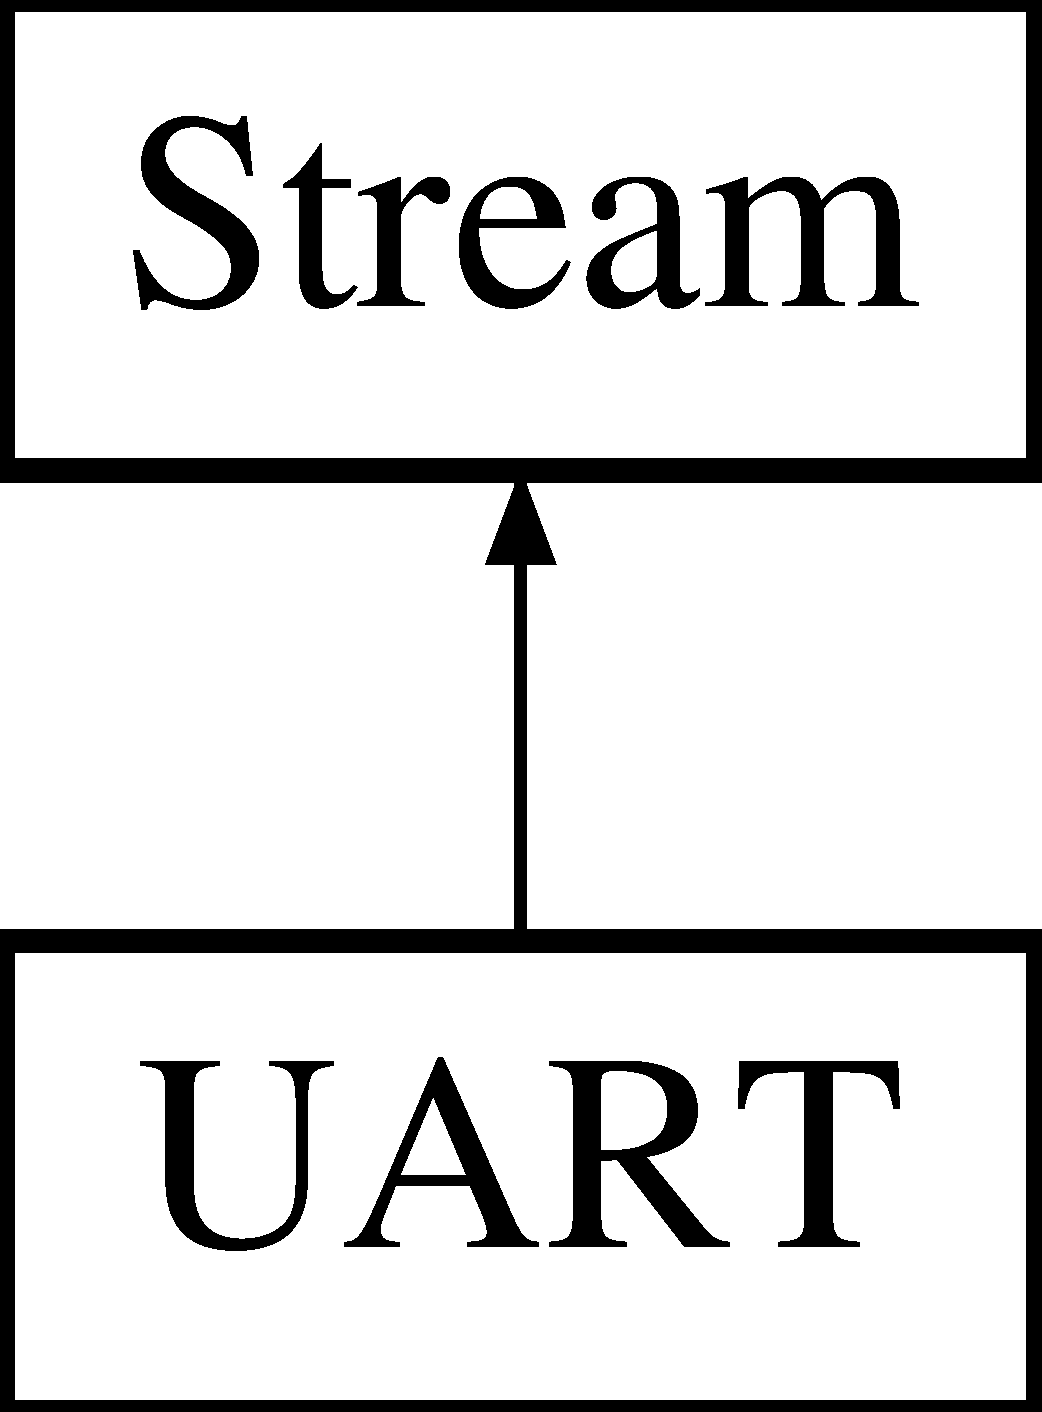
\includegraphics[height=2.000000cm]{class_u_a_r_t}
\end{center}
\end{figure}
\subsection*{Public Member Functions}
\begin{DoxyCompactItemize}
\item 
void \hyperlink{class_u_a_r_t_a8bb77ca27b4e17d608d2743313625ac4}{Write} (uint8\-\_\-t $\ast$string, uint16\-\_\-t size)
\item 
void \hyperlink{class_u_a_r_t_aed659ee8bc31ba966144d1a522506a7b}{Init} (uint16\-\_\-t baud\-\_\-rate)
\item 
\hyperlink{class_u_a_r_t_a97debffc29b178c09b104f4542298a36}{U\-A\-R\-T} (const \hyperlink{class_u_a_r_t}{U\-A\-R\-T} \&)=delete
\item 
void \hyperlink{class_u_a_r_t_a843ab7fc20f5ce5f030d2ca5ee98d6b6}{operator=} (const \hyperlink{class_u_a_r_t}{U\-A\-R\-T} \&)=delete
\end{DoxyCompactItemize}
\subsection*{Static Public Member Functions}
\begin{DoxyCompactItemize}
\item 
static \hyperlink{class_u_a_r_t}{U\-A\-R\-T} \& \hyperlink{class_u_a_r_t_a745c8f35f3ca3ab6359cedda3e640777}{Get\-Instance} ()
\end{DoxyCompactItemize}
\subsection*{Private Member Functions}
\begin{DoxyCompactItemize}
\item 
\hypertarget{class_u_a_r_t_a195cdcca08c2ae1d03ee8bf13a87b95a}{void {\bfseries initialize\-\_\-transmission} ()}\label{class_u_a_r_t_a195cdcca08c2ae1d03ee8bf13a87b95a}

\item 
\hyperlink{class_u_a_r_t_a68e7e88d2a13f5da85f0fde1ef98515f}{U\-A\-R\-T} ()
\end{DoxyCompactItemize}
\subsection*{Private Attributes}
\begin{DoxyCompactItemize}
\item 
\hypertarget{class_u_a_r_t_ae98e7d277a1833478aa85dc9e686150a}{bool {\bfseries ongoing\-\_\-transmission} = false}\label{class_u_a_r_t_ae98e7d277a1833478aa85dc9e686150a}

\end{DoxyCompactItemize}
\subsection*{Friends}
\begin{DoxyCompactItemize}
\item 
void \hyperlink{class_u_a_r_t_accc13d37cd82c841e387e1d5cf4d9a94}{U\-S\-A\-R\-T0\-\_\-\-U\-D\-R\-E\-\_\-vect} ()
\end{DoxyCompactItemize}
\subsection*{Additional Inherited Members}


\subsection{Constructor \& Destructor Documentation}
\hypertarget{class_u_a_r_t_a97debffc29b178c09b104f4542298a36}{\index{U\-A\-R\-T@{U\-A\-R\-T}!U\-A\-R\-T@{U\-A\-R\-T}}
\index{U\-A\-R\-T@{U\-A\-R\-T}!UART@{U\-A\-R\-T}}
\subsubsection[{U\-A\-R\-T}]{\setlength{\rightskip}{0pt plus 5cm}U\-A\-R\-T\-::\-U\-A\-R\-T (
\begin{DoxyParamCaption}
\item[{const {\bf U\-A\-R\-T} \&}]{}
\end{DoxyParamCaption}
)\hspace{0.3cm}{\ttfamily [delete]}}}\label{class_u_a_r_t_a97debffc29b178c09b104f4542298a36}
Beacause of singleton -\/ makes sure its not copied etc. \hypertarget{class_u_a_r_t_a68e7e88d2a13f5da85f0fde1ef98515f}{\index{U\-A\-R\-T@{U\-A\-R\-T}!U\-A\-R\-T@{U\-A\-R\-T}}
\index{U\-A\-R\-T@{U\-A\-R\-T}!UART@{U\-A\-R\-T}}
\subsubsection[{U\-A\-R\-T}]{\setlength{\rightskip}{0pt plus 5cm}U\-A\-R\-T\-::\-U\-A\-R\-T (
\begin{DoxyParamCaption}
{}
\end{DoxyParamCaption}
)\hspace{0.3cm}{\ttfamily [private]}}}\label{class_u_a_r_t_a68e7e88d2a13f5da85f0fde1ef98515f}
A constructor that initializes the \hyperlink{class_u_a_r_t}{U\-A\-R\-T} to a certain size 

\subsection{Member Function Documentation}
\hypertarget{class_u_a_r_t_a745c8f35f3ca3ab6359cedda3e640777}{\index{U\-A\-R\-T@{U\-A\-R\-T}!Get\-Instance@{Get\-Instance}}
\index{Get\-Instance@{Get\-Instance}!UART@{U\-A\-R\-T}}
\subsubsection[{Get\-Instance}]{\setlength{\rightskip}{0pt plus 5cm}static {\bf U\-A\-R\-T}\& U\-A\-R\-T\-::\-Get\-Instance (
\begin{DoxyParamCaption}
{}
\end{DoxyParamCaption}
)\hspace{0.3cm}{\ttfamily [inline]}, {\ttfamily [static]}}}\label{class_u_a_r_t_a745c8f35f3ca3ab6359cedda3e640777}
A Singleton implementation of this class \hypertarget{class_u_a_r_t_aed659ee8bc31ba966144d1a522506a7b}{\index{U\-A\-R\-T@{U\-A\-R\-T}!Init@{Init}}
\index{Init@{Init}!UART@{U\-A\-R\-T}}
\subsubsection[{Init}]{\setlength{\rightskip}{0pt plus 5cm}void U\-A\-R\-T\-::\-Init (
\begin{DoxyParamCaption}
\item[{uint16\-\_\-t}]{baud\-\_\-rate}
\end{DoxyParamCaption}
)}}\label{class_u_a_r_t_aed659ee8bc31ba966144d1a522506a7b}
Initializer because of the singleton implementation. 
\begin{DoxyParams}{Parameters}
{\em baud\-\_\-rate} & The baud rate of the uart \\
\hline
\end{DoxyParams}
\hypertarget{class_u_a_r_t_a843ab7fc20f5ce5f030d2ca5ee98d6b6}{\index{U\-A\-R\-T@{U\-A\-R\-T}!operator=@{operator=}}
\index{operator=@{operator=}!UART@{U\-A\-R\-T}}
\subsubsection[{operator=}]{\setlength{\rightskip}{0pt plus 5cm}void U\-A\-R\-T\-::operator= (
\begin{DoxyParamCaption}
\item[{const {\bf U\-A\-R\-T} \&}]{}
\end{DoxyParamCaption}
)\hspace{0.3cm}{\ttfamily [delete]}}}\label{class_u_a_r_t_a843ab7fc20f5ce5f030d2ca5ee98d6b6}
Beacause of singleton -\/ makes sure its not copied etc. \hypertarget{class_u_a_r_t_a8bb77ca27b4e17d608d2743313625ac4}{\index{U\-A\-R\-T@{U\-A\-R\-T}!Write@{Write}}
\index{Write@{Write}!UART@{U\-A\-R\-T}}
\subsubsection[{Write}]{\setlength{\rightskip}{0pt plus 5cm}void U\-A\-R\-T\-::\-Write (
\begin{DoxyParamCaption}
\item[{uint8\-\_\-t $\ast$}]{string, }
\item[{uint16\-\_\-t}]{size}
\end{DoxyParamCaption}
)\hspace{0.3cm}{\ttfamily [virtual]}}}\label{class_u_a_r_t_a8bb77ca27b4e17d608d2743313625ac4}
Write the inserted string to output (i.\-e. write to computer) 
\begin{DoxyParams}{Parameters}
{\em string} & The \char`\"{}data string\char`\"{} that shall be written to the output \\
\hline
{\em size} & the size of the data string \\
\hline
\end{DoxyParams}


Reimplemented from \hyperlink{class_stream_a508be3423e4d99ab2757275fb723002a}{Stream}.



\subsection{Friends And Related Function Documentation}
\hypertarget{class_u_a_r_t_accc13d37cd82c841e387e1d5cf4d9a94}{\index{U\-A\-R\-T@{U\-A\-R\-T}!U\-S\-A\-R\-T0\-\_\-\-U\-D\-R\-E\-\_\-vect@{U\-S\-A\-R\-T0\-\_\-\-U\-D\-R\-E\-\_\-vect}}
\index{U\-S\-A\-R\-T0\-\_\-\-U\-D\-R\-E\-\_\-vect@{U\-S\-A\-R\-T0\-\_\-\-U\-D\-R\-E\-\_\-vect}!UART@{U\-A\-R\-T}}
\subsubsection[{U\-S\-A\-R\-T0\-\_\-\-U\-D\-R\-E\-\_\-vect}]{\setlength{\rightskip}{0pt plus 5cm}void U\-S\-A\-R\-T0\-\_\-\-U\-D\-R\-E\-\_\-vect (
\begin{DoxyParamCaption}
{}
\end{DoxyParamCaption}
)\hspace{0.3cm}{\ttfamily [friend]}}}\label{class_u_a_r_t_accc13d37cd82c841e387e1d5cf4d9a94}
The interrupt handler vector. To be run on each D\-R\-E interrupt 

The documentation for this class was generated from the following files\-:\begin{DoxyCompactItemize}
\item 
lib/uart/\hyperlink{uart_8h}{uart.\-h}\item 
lib/uart/uart.\-cpp\end{DoxyCompactItemize}

\chapter{File Documentation}
\hypertarget{oled_8h}{\section{lib/oled/oled.h File Reference}
\label{oled_8h}\index{lib/oled/oled.\-h@{lib/oled/oled.\-h}}
}
{\ttfamily \#include \char`\"{}../stream/stream.\-h\char`\"{}}\\*
{\ttfamily \#include $<$avr/io.\-h$>$}\\*
\subsection*{Classes}
\begin{DoxyCompactItemize}
\item 
class \hyperlink{class_o_l_e_d}{O\-L\-E\-D}
\end{DoxyCompactItemize}


\subsection{Detailed Description}
\begin{DoxyAuthor}{Author}
Johan Lofstad, Sondre Baugstø and Sondre Russvoll 
\end{DoxyAuthor}
\begin{DoxyVersion}{Version}
1.\-0
\end{DoxyVersion}
An interface to communicate with the oled display 
\hypertarget{stream_8h}{\section{lib/stream/stream.h File Reference}
\label{stream_8h}\index{lib/stream/stream.\-h@{lib/stream/stream.\-h}}
}
{\ttfamily \#include $<$string.\-h$>$}\\*
{\ttfamily \#include $<$avr/io.\-h$>$}\\*
\subsection*{Classes}
\begin{DoxyCompactItemize}
\item 
class \hyperlink{class_stream}{Stream}
\end{DoxyCompactItemize}


\subsection{Detailed Description}
\begin{DoxyAuthor}{Author}
Johan Lofstad, Sondre Baugstø, Sondre Russvoll 
\end{DoxyAuthor}
\begin{DoxyVersion}{Version}
1.\-0
\end{DoxyVersion}
An interface for handling streams with default methods. 
\hypertarget{uart_8h}{}\section{lib/uart/uart.h File Reference}
\label{uart_8h}\index{lib/uart/uart.\+h@{lib/uart/uart.\+h}}
{\ttfamily \#include $<$avr/io.\+h$>$}\newline
{\ttfamily \#include $<$avr/interrupt.\+h$>$}\newline
{\ttfamily \#include \char`\"{}../stream/stream.\+h\char`\"{}}\newline
\subsection*{Classes}
\begin{DoxyCompactItemize}
\item 
class \hyperlink{class_u_a_r_t}{U\+A\+RT}
\end{DoxyCompactItemize}
\subsection*{Macros}
\begin{DoxyCompactItemize}
\item 
\hypertarget{uart_8h_a711e9130c825a7269c8c87dbb57a85e0}{}\label{uart_8h_a711e9130c825a7269c8c87dbb57a85e0} 
\#define {\bfseries M\+Y\+U\+B\+RR}~F\+O\+SC/16/B\+A\+UD-\/1
\end{DoxyCompactItemize}
\subsection*{Functions}
\begin{DoxyCompactItemize}
\item 
\hypertarget{uart_8h_a95e67e677722a53e3ad9f1ffce2e7408}{}\label{uart_8h_a95e67e677722a53e3ad9f1ffce2e7408} 
{\bfseries I\+SR} (U\+S\+A\+R\+T0\+\_\+\+U\+D\+R\+E\+\_\+vect)
\end{DoxyCompactItemize}


\subsection{Detailed Description}
\begin{DoxyAuthor}{Author}
Johan Lofstad, Sondre Baugstø and Sondre Russvoll 
\end{DoxyAuthor}
\begin{DoxyVersion}{Version}
1.\+1
\end{DoxyVersion}
An interface for communicating through \hyperlink{class_u_a_r_t}{U\+A\+RT} 
%--- End generated contents ---

% Index
\backmatter
\newpage
\phantomsection
\clearemptydoublepage
\addcontentsline{toc}{chapter}{Index}
\printindex

\end{document}
